%!TeX program=pdflatex
%!TeX encoding=utf8
%!TeX spellcheck = en_US
%!TeX root = ../../messageVortex.tex


% ********************************************************************************************************
% *** Methodes
% ********************************************************************************************************
\part{Methodes}
In this part of the thesis we collect requirements, definitions, methods, and existing research relevant to the topic of this thesis. We start with collecting requirements for the protocol. 

Having the requirements we collect numerous existing technologies on research and implementation level. Each of the technologies is quickly categorized and either further studied or rejected naming the reasons for rejection.

The list of technologies and research collected is big in this chapter. All relevant technologies either widely adopted or thoroughly researched should be included in this chapter. All Technologies and research are categorized. 

Technologies are always referenced through their respective standard. If applicable multiple standards may be part of the analysis. A very quick introduction into the protocol is given and then analysed for suitability for a specific problem addressed in this work.

Research are referenced by a paper. If applicable multiple related researches and papers are collected together into a bigger picture an then analysed for suitability concerning specific problem. If related to a standard technology links to that technology are provided where relevant.

In chapter \ref{sec:genRequirements} we collect the requirements for the protocol. Based on findings in this section we collect in chapter \ref{sec:existingTPP}. In chapter \ref{sec:existingRD} we collect relevant research to the topic. In chapter \ref{sec:appliedMethods} we summarize the identified  methods which will be used. We explain choices and give a rough outline of the protocol baselines.

\chapter{Requirements for an anonymising Protocol\label{sec:genRequirements}}
In the following sections we try to elaborate the main characteristics of the anonymising protocol. 

The main goal of the protocol is to enable Freedom of speech as defined in Article 19 of the International Covenant on Civil and Political Rights (ICCPR)\cite{iccpr}.
\begin{quote}
	everyone shall have the right to hold opinions without interference 
\end{quote}
and
\begin{quote}
	everyone shall have the right to freedom of expression; this right shall include freedom to seek, receive and impart information and ideas of all kinds, regardless of frontiers, either orally, in writing or in print, in the form of art, or through any other media of his choice.
\end{quote}

We imply that not all participants in the internet share this value. As of September \nth{1} 2016 Countries such as China (signatory), Cuba (signatory), Quatar, Saudi Arabia, Singapore, United Arab Emirates, or Myanmar did not ratify the ICCPR. Other countries such as United States or Russia did either put local laws in place superseding the ICCPR or made reservations rendering parts of it ineffective. We may therefore safely assume that freedom of speech is not given in the internet as a lot of countries explicitly supersede them.

Network packets may pass though any point of the world. A sender has no control over it since every routing device decides on its own for the next hop. This decision may be based on static rules or influenced by third party nodes or circumstances (e.g., BGB, RIP, OSPF\ldots). It is furthermore not possible to detect what way has a packet taken. The common network diagnostic tool \verb|tracert| respectively \verb|traceroute| list a possible list of hops. This list is only correct under certain circumstances (e.g., stable route for multiple packets, or equal routing decisions regardless of other properties than source and destination address) and may not be used as prof of routing decisions. Neither can a route of a packet beeing sent forseen nor can it be measured while or after sending. 

As an example of the problems analysing a packet route we may look at \verb|traceroute|. The mapage of traceroute of Linux tells us that \verb|traceroute| uses UDP, TCP, or ICMP packets with a short TTL and analyses the IP of the peer sending an TIME\_EXCEEDED (message of the ICMP protocol). This information is then collected and shown as a route. This route may be completely wrong. Some of the possible cases are described in the manpage.

We cannot be sure that data packets we are sending are passing only through countries accepting the ICCPR to the full extend.

\begin{figure}[H]
	\begin{lstlisting}[language=bash,breaklines=true,basicstyle=\tiny]
$ traceroute www.ietf.org
traceroute to www.ietf.org.cdn.cloudflare-dnssec.net (104.20.0.85), 64 hops max
1   147.86.8.253  0.418ms  0.593ms  0.421ms
2   10.19.0.253  1.177ms  0.829ms  0.782ms
3   10.19.0.253  0.620ms  0.427ms  0.402ms
4   193.73.125.35  1.121ms  0.828ms  0.905ms
5   193.73.125.81  2.991ms  2.450ms  2.414ms
6   193.73.125.81  2.264ms  1.961ms  1.959ms
7   192.43.192.196  6.472ms  199.543ms  201.152ms
8   130.59.37.105  3.465ms  3.138ms  3.121ms
9   130.59.36.34  3.904ms  3.897ms  4.989ms
10   130.59.38.110  3.625ms  3.333ms  3.379ms
11   130.59.36.93  7.518ms  7.232ms  7.246ms
12   130.59.38.82  7.155ms  17.166ms  7.034ms
13   80.249.211.140  22.749ms  22.415ms  22.467ms
14   104.20.0.85  22.398ms  22.222ms  22.146ms
	\end{lstlisting}
	\caption{A traceroute to the host www.ietf.org}
\end{figure}

\section{Adversary model\label{sec:adversary}}
For an anonymizing adversary we need to assume someone of the capabilities of a state sponsored actor. State sponsored actors may work these days with allies but will not achieve dominance over all jurisdictional domains.

For our adversary modell we assume the following properties:
\begin{itemize}
	\item An adversary will have technical knowhow to attack any infrastructure.
	\item An adversary may have the capability to monitor traffic at any point in any network within a juridiction.
	\item An adversary may have the capability to freely modify routing information within a juridiction.
	\item An adversary may have the possibility to freely modify even cryptographically strong secured data where a single or a limited number of entities grant any kind of proof of authenticity or privacy.
	\item An adversary may have the possibility to inject or modify any data on the network of a jurisdiction.
	\item An adversary may create own nodes of a network and monitor their behaviour and data flow to the maximum possible extent.
	\item An adversary may force other non-allied nodes to expose their data to him.
	\item An adversary may have the same access to resources as within its jurisdiction in a limited number of other jurisdictions.
\end{itemize}

We assume the following goals for an adversary:
\begin{itemize}
	\item An adversary may want to disrupt non-authorized communication.
	\item An adversary may want to read any information passing throughout the internet.
	\item An adversary may want to build and conserve data about individuals or groups of individuals of their live. This data includes all activities in any part of their live regardless of their obvious fitness for any specific purpose.
\end{itemize}

\section{Required Properties}

\subsection{Anonymizing and Unlinking}
If we are unable to limit the route of our packets through named jurisdictions we must protect ourselves from unintentionally breaking the law of a foreign country. Therefore we need to be anonymous when sending or receiving messages. Unfortunately most transport protocols (in fact almost all of them such as SMTP, SMS, XMPP, or IP) use a globally unique identifier for senders and receivers which are readable by any party which is capable of reading the packets. 

As a result anonymisation of a sender or a receiver is not simple. If messages are being sent through a relay at least the original sender might be concealed. By combining it with encryption we may even achieve a very simple form of sender and Receiver Pseudonymity. If cascading more relay like infrastructures and combining it with cryptography we might even achieve sender and receiver anonymity. This approach has however several downsides (see \ref{sec:remailer} and \ref{sec:mixnets} for details) and is easily attackable.

\subsection{Censorship Resistant}
In our scenario in \ref{sec:genRequirements} we defined the adversary as someone with superior access to the internet and its infrastructure. Such an adversary might attack a message flow in several ways:
\begin{itemize}
	\item Identify sender
	\item Identify recipient
	\item Read messages passed or extract meta information
	\item Disrupt communication fully or partially
\end{itemize}

We furthermore have to assume that all actions taken by a potential adversary are not subject to legal prosecution. This is due to the fact that an adversary trying to establish censorship may be part of a jurisdictions government. We may safely assume that there are legal exceptions in some jurisdiction for such entities.

In order to be able to withstand an adversary outlined above the protocol needs certain attributes. The message content needs to be unidentifiable by attributes or content. Whereas ``Attributes'' include meta information such as frequency, timing, message size, sender, protocol, ports, or recipient (list not conclusive).

\subsection{Controllable trust}
If we want to control trust we have to conclude that
\begin{enumerate}
	\item trust in an infrastructure is given due to the fact that it is under full control of either the sender or the recipient.
	\item trust in an infrastructure may not be necessary as the infrastructure is ideally unable to misuse data passed through it.
\end{enumerate}
In this thesis we work with both cases. We will however never trust a third party apart from sender and recipient (not even their providers of infrastructures).

\subsection{Reliable}
Any message sending protocol needs to be reliable in its functionality. If means of message transport are unreliable users tend to use different means for communication. 

\subsection{Diagnosable}
Reliability is somehow linked to transparent behaviour. This due to the fact that if something is generating a constant behaviour but we are unable to determine the reason for it (i.e. if we are expecting a different behaviour) we normally assume a malfunction. Therefore ``Reliable'' means not only stable by its behaviour. It means also diagnosable. User perception will not be ``Reliable'' if he is not able to determine causes for differences in observed and expected behaviour.

\subsection{Available}
Availability has two meanings in this context which do differ. A technology is available if\ldots
\begin{enumerate}
	\item a sender and a recipient have (or may have) the means of using it.
	\item the infrastructure is providing the service (as opposed to: ``is running in a degraded/faulty state unable to provide a service).
\end{enumerate}

The first meaning tells us that a protocol must run independently from infrastructure the user has commonly ready.

The second meaning tells us that messages must always be capable of flowing from the sender to the recipient. As infrastructure may fail at any time the protocol must offer the possibilities to send messages through alternate routes. This sounds easy and many protocols implement such redundancies already. However, taking into account that sender and recipient is not known to a routing node this is a goal hard to achieve.

\section{Rough draft of Protocol Layers}
In order to fulfil the criteria given above we define a very rough idea of the protocol and its layers. The rough overview is given in figure \ref{fig:roughProtocolDesign}. The protocol should work on the base of onion routing. Unlike Tor (see \ref{sec:tor}) it should not rely on central infrastructures. it furthermore should not be limited to onionize messages. It should be capable of splitting and reassemble messages at any layer 

\begin{figure}[h]
	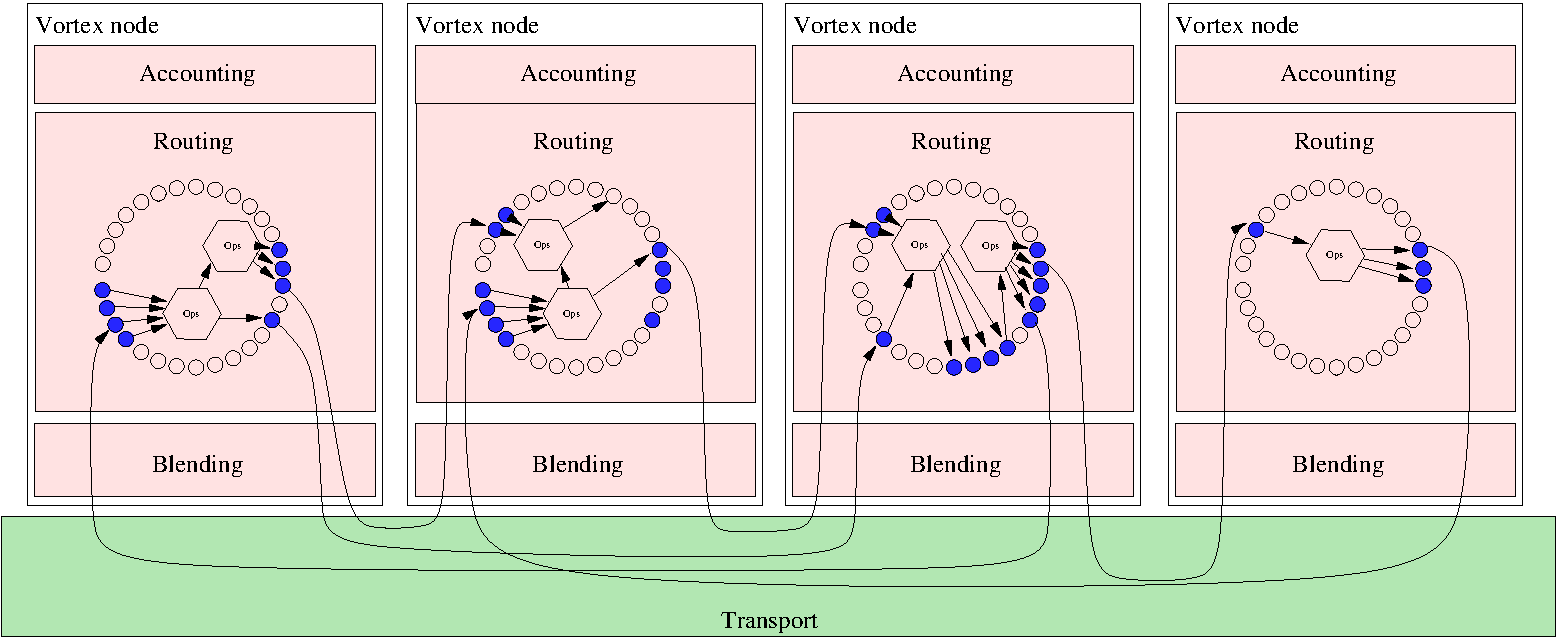
\includegraphics[width=\columnwidth]{inc/roughProtocolDesign.pdf}
	\caption{A first rough overview for the protocol}
	\label{fig:roughProtocolDesign}
\end{figure}	

The protocol itself should send messages through a well known transport protocol (``Transport'') which will be used for our messages. 

The messages will be hidden within regular messages already using that transport layer. In an ideal implementation messages sent by our protocol should be indistinguishable from regular messages (by computers and humans). In order to achieve this particular task we introduce a ``Hiding / Blending'' layer. This layer is normally specific to the underlying transport layer and may vary.

The ``Routing'' layer is the layer that receives and sends messages. It parses only the core protocol and the data processed here is completely independent from the underlying transport layer.

The ``Assembly / Accounting'' layer disassembles the received messages into its parts. It then recomposes and stores the messages for further routing. In order to avoid spaming over this media some kind of accounting will be involved. 

The messages passed through such a protocol stack are ononised to offer anonymity from evil nodes. Furthermore a node should be unable to tell whether a message was intended for a specific node or not (so all nodes including sender and recipient should handle identically).

In order to mitigate size based attacks (an onionised packet looses permanently data on its way) we introduce operations which may be applied to a valid message as well as to decoy traffic. The operations should be able to increase and decrease in size without being able to tell if this message is destined to a target or not. Operations not carried out due to missing data might be either intentionally or a malfunction.

The defined message operations are as follows:
\begin{itemize}
	\item Split a message block into two parts of variable size.\\
	This operation may be used to fan out decoy traffic, to cut off decoy data, or to send multiple parts of a message through diffferent routing nodes.
	\item Join two data blocks to a bigger block using an xor operation.\\
	This operation may be used to minimise decoy traffic or to rejoin data which has been split earlier.
	\item Fork off xor'ed data from a data block by applying an xor operation to a received block with a block of random data.\\
	With this operation we may create decoy traffic, or split a message into two parts.
	\item Encrypt a block with a given key.      
	\item Decrypt a block with a given key.
\end{itemize}

To avoid making this system attractive to UBE an accounting system is introduced. The system works as follows:
\begin{itemize}
	\item Routing nodes may offer their services at a cost. These ``costs'' are typically paid by solving crypto puzzles.
	\item The following operations may be cost effective:
	\begin{itemize}
		\item Getting a discardable identity on a node (prerequisite for accounting).
		\item Allowance to route a number of messages through the node (cost per outgoing message) in a specified interval. This allowance is always linked to a discardable identity.
		\item Allowance to route a specific size of bytes through the node (cost per outgoing byte) in a specified time interval. This allowance is always linked to a discardable identity.
		\item Offer information about the known routing network by the node.
		\item Offer information about the identities current quota.
	\end{itemize}
\end{itemize}
All quotas require accounting. In order to minimise accounting all these quotas must be assigned a time interval in which they are effective. this guarantees that quota data is not growing indefinitely. It is up to the node to decide what time duration is still acceptable.

In order to limit the possibility to Denial of Service (DoS) a node by overloading it the following precautions are taken:
\begin{itemize}
	\item The message is built in such a way that message building is far more complex than message routing.
	\item Messages may be decrypted in parts to minimize the amount of work required to decide whether the full processing of the message will be done or the message is discarded anyway.
	\item The usage of inefficient operations (e.g. asymmetric encryption) is minimized.
	\item The server may limit specific operations.
\end{itemize}

\section{Rough Draft of Messages}
For our protocol we assume the following outline for a message:
\begin{itemize}
	\item Header block\\ 
	This block contains an ephemeral identity of the sender on the message processing host. It allows the host to decide wether he is willing to process the rest of the message or not. It is important to know that the identity block contains a symmetric key for decryption of the main block and a secret repeated in the main block. This prevents that a malicious node may exchange the main block.
	\item Main block\\
	This block contains all information regarding routing and processing data. It furthermore contains the payload data which may or may not contain messages.
	\begin{itemize}
		\item Routing Blocks\\
		This block contains information of which data block should be sent to what recipient. It furthermore may contain instruction for processing the data blocks and routing/reply blocks for subsequent processing. Another important thing to note is that routing blocks and payload data may arrive on two different paths to the target node.
		\item Routing Log Block\\
		This Block contains information about the already occurred routing in onionised form. It may be regarded as the onionised pendant of received header in an SMTP header.
		\item Reply Block\\
		This Block contains a Routing block which may be used to contact the original sender of a message (e.g. for an error message)
		\item payload Block\\
		These Blocks form the payload data. It might contain a message, parts of a message or decoy material.
	\end{itemize}      
\end{itemize}

The message is picked up from the transport layer and extracted in the blending layer. Processing is then split. First the Assembly/accounting layer is extracting the identity block and authorises further processing. The message building instructions are put into a identity specific list (with the expiration dates of the message). and the payload blocks are stored (again with the expiration date). 

After having prepared the message in such a way the routing layer gets the routing blocks. Every routing block is then processed after a final approval by the accounting layer (he is in charge to keep the quotas for this identity in  sync). The routing layer assembles the new messages according to the (no authorized) instructions in the routing block and sends it to the next hop where the processing restarts with the new instructions. 

\chapter{Existing Transport Layer Protocols \label{sec:existingTPP}}
In this chapter we have a look at various available transport layer protocol. The main goal is to identify strong candidates as a transport layer. Main focus lies on the following criterias:
\begin{itemize}
	\item Widely adopted (Ct1)\\
	The more widely adopted and used a protocol is the harder it is for an adversary to monitor (due to the sheer mass), filter or block the protocol (censorship resistance).
	\item Reliable (Ct2)\\
	Message transport between peers should be reliable. As messages may arrive anytime from everywhere we don not have means to synchronize the peer partners on a higher level without investing a considerable effort. In order to avoid this effort we do look for inherently reliable protocols.
	\item Symmetrical built (Ct3)\\
	The transport layer should be built on a peer to peer base. All servers implement a generic routing which requires no prior knowledge of possible targets. This criteria neglects centralised infrastructures.
\end{itemize}

Ct3 may be dropped if assuming that routing is done by the blending layer, or a specialized transport layer.



\section{Roundup for Transport Protocols}
\begin{table}[h]
	\centering\tiny
	\begin{tabular}{|l|l|l|l|}\hline
		\diaghead{\theadfont protocol Criteria}{Protocol}{Criteria} & \thead{Ct1: Widely adopted} 	& \thead{Ct2: Reliable} & \thead{Ct3: Symmetrically built}\\\hline
		HTTP	 & $\checkmark$			& $\checkmark$		& $\times$\\              
		FTP		 & $\checkmark$			& $\checkmark$		& $\times$\\
		TFTP     & $\times$				& $\times$			& $\times$\\
		MQTT	 & \textasciitilde		& $\checkmark$		& $\times$\\              
		AMQP	 & \textasciitilde		& $\checkmark$		& $\times$\\
		CoAP	 & \textasciitilde		& \textasciitilde 	& $\times$\\
		WAMP	 & $\times$				& $\checkmark$		& \textasciitilde\\
		XMPP	 & $\checkmark$			& $\checkmark$		& $\checkmark$\\
		SMTP	 & $\checkmark$			& $\checkmark$		& $\checkmark$\\
		SMS\footnotemark[1] & 			& 					& \\
		MMS		 & $\times$			    & $\checkmark$		& $\times$\\\hline
	\end{tabular}	
	\caption{comparison of protocols in terms of the suitability criteria as transport layer}
	\label{tab:protoSuitCrit}
\end{table}

In table \ref{tab:protoSuitCrit} we sum up all previously analysed protocols. We use ``$\checkmark$'' for a fulfilled criteria, ``\textasciitilde'' for a partially fulfilled criteria, and ``$\times$'' for a not fulfilled criteria. This overview shows in compact form which protocols have been identified as strong candidates for use as a transport layer in terms of an anonymising protocol. 

This table shows that strong identified candidates are SMTP (being already a message sending protocol on asynchronous base) and XMPP (a real time chat protocol able to attach files. This protocol features furthermore end-to-end encryption and signing). Both have the advantages that they are really wide adopted in the internet and do support additionally advanced content (such as alternatives or attachments).

\footnotetext[1]{omitted due to message size being too small}

If assuming an implemented transport layer on the MessageVortex protocol side, HTTP and FTP may be considered valid candidates as well.


\chapter{Existing Research and Implementations on the Topic \label{sec:existingRD}}
\section{Anonymity}
\DeclareFixedFootnote{\omitted}{footnotes omitted in quote}
As Anonymity we take the definition as specified in \cite{anon_terminology}.
\begin{quote}
	Anonymity of a subject means that the subject is not identifiable within a set of subjects, the anonymity set.\omitted
\end{quote}
and
\begin{quote}
	Anonymity of a subject from an attacker's perspective means that the attacker cannot sufficiently identify the subject within a set of subjects, the anonymity set.\omitted
\end{quote}

Whereas the anonymity set is defined as the set of all possible subjects.

Especially the anonymity of a subject from an attacker's is very important to this paper. 

\subsection{$k$-Anonymity}
$k$-anonymity is a term introduced in \cite{k-anonymous:ccs2003}. This work claims that no one might be held responsible for an action if the action itself can only be identified as an action which has been taken by one unidentifiable entity out of $k$ entities.

The Document distinguishes between \textit{Sender $k$-anonymity} where the sending entity can only be narrowed down to a set of $k$ entities and \textit{Receiver $k$-anonymity}. 

The size of $k$ is a key factor. One of the criteria might be the legal requirements of a jurisdiction. Depending on the jurisdiction it is normally not possible prosecute someone if an action is not directly coupled to one person. Another criteria might be the decreasing of $k$ over time. If a Vortex account is used we have to assume that some vortex identities go out of commission over time. If $k$ is chosen according to a legal requirement it should be taken into account that $k$ might be decreasing over time.

\subsection{$\ell$-Diversity}
In \cite{machanavajjhala2007diversity} an extended model of $k$-anonymity is introduced. In this paper the the authors emphasize that it is possible to break a $k$-anonymity set if there is additional Information available which may be merged into a data set so that a special entity can be filtered from the $k$-anonymity set. In other words if an anonymity set is to tightly specified a single additional background information might be sufficient to identify a specific entity in an anonymity set.

While it might be arguable that a $k$-anonymity in which a member is not implicitely $k$-anonymous still is sufficient for $k$-anonymity in its sense the point made in this work is definitely right and should be taken into account.

Their approach is to introduce an amount of invisible diversity into $k$-anonymous sets so that simple background knowledge is no longer sufficient to isolate a single member.

\subsection{$t$-Closeness}
While $\ell$-diversity protects the identity of an entity it does not prevent information gain. A subject which is in a class has the same attributes. This is where $t$-closeness\cite{li2007t} comes into play. $t$-closeness is defined as follows:

\begin{quote}
	An equivalence class is said to have $t$-closeness if the distance between the distribution of a sensitive attribute in this class and the distribution of the attribute in the whole table is no more than a threshold. A table is said to have $t$-closeness if all equivalence classes have $t$-closeness.
\end{quote}

\subsection{Ephemeral Identity}
In this work we use accounting on various levels. While we are dealing with anonymity accounting has still to be linked to some kind of identity for this reason we are introducing a term called ``ephemeral identity''.

\begin{quote}
	A Ephemeral identity is a temporary identity which is defined by the following attributes:
	\begin{itemize}
		\item It is an artificial identity
		\item It is only used for a short timespan
		\item It is not linkable to another identity
	\end{itemize}
\end{quote}

The key in this definition is the last point is crucial and at the same time hard to achieve.

\section{Single Use Reply Blocks and Multi Use Reply Blocks}
The use of single use reply blocks were first introduced by Chaum in \cite{CHAUM1}. A routing block in general is a structure allowing to send a message to someone without knowing the targets true address. It might be differentiated into ``Single Use Reply Bolcks'' (SURBs) which may be used once and ``Multi Use Reply Blocks'' (MURBs) which may be used a limited number of times. 

The concept is that we have in our case a routing block which might be used up to $n$ times ($0<n<127$). The number has been chosen for practical reasons. It is easily representable in a byte integer (signed or unsigned) on any system. It is big enough to support human communication in a sensible way and is big enough to add not too much overhead when rerequesting more MURBs. The number should not be too big because if a MURB is reused the same pattern of traffic is generated thus making the system susceptible to statistical attacks.

\section{Censorship}
As definition for censorship we take
\begin{quote}
	Censorship: the cyclical suppression, banning, expurgation, or editing by an individual, institution, group or government that enforce or influence its decision against members of the public -- of any written or pictorial materials which that individual, institution, group or government deems obscene and "utterly without redeeming social value," as determined by "contemporary community standards.".
\end{quote}
Which is attributed to Chuck Stone Professor at the School of Journalism and Mass Communication, University of North Carolina. Please note that ``Self Censorship'' (not expressing something in fear of consequences) is a form of censorship too.

In our more technical subsystem this means
\begin{quote}
	A systematic suppression, modification, or banning of data in the internet by either removal, or modification of the data, or systematic influencing of entities involved in the processing (e.g. by writing, routing, storing or reading) of this data.
\end{quote}

\subsection{Censorship Resistant}
A censorship resistant system is a system which allows the users of the system and the data itself to be unaffected from censorship. Please note that this does not deny the possibility of censorship per se. It still exists outside the system. But it has some consequences for the system itself.

\begin{itemize}
	\item The system must be either undetectable or out of reach for an entity censoring.\\
	The possibility of identifying a protocol or data allows a censoring entity to suppress the use of the protocol itself. 
	\item The entities involved in a system must be untraceable.\\
	Traceable entities would result in means of suppressing real world entities participating in the system.
\end{itemize}

\subsection{Parrot Circumvention}
In \cite{oakland2013-parrot} \citeauthor{oakland2013-parrot} express that it is easy for a human to determine decoy traffic as the content is easily identifiable as automated content. While this is absolutely true there is a possibility here to generate ``human like'' data traffic to a certain extent. In our design this is the job covered by the blending layer.

\subsection{Censorship Circumvention}
Several technical ways have been explored to circumvent censorship. All seem to boil down to two main ideas:
\begin{itemize}
	\item Hide data.
	\item Copy data to a vast amount of places in order to improve the lifespan of data.
\end{itemize}

In the following section we look at technologies and ideas dealing with these circumvention technologies.

\subsubsection{Covert Channel and Channel Exploitations}
The original term of covert channels was defined by \citeauthor{Lampson73anote}\cite{Lampson73anote} as 
\begin{quote}
	not intended for information transfer at all, such as the service program's effect on system load.
\end{quote}

This was defined  in such a way to distinguish the message flow from 
\begin{quote}
	legitimate channels used by the confined service, such as the bill.
\end{quote}

The use of a legitimate channel such as SMTP and hide information in this specific channel is not a usage of covert channel. This methode is commonly referenced as channel exploitation.

\subsubsection{Steganography}
Steganography is an important part when it comes to unlinking information. In \cite{6828087} and \cite{subhedar2014current} we get a very rough overview. As some of the types and algorithms address specific topics of steganography (e.g., some hide from automatic detection and others address a human message stream auditor), we need to carefully choose. In our specific case the main idea is to hide within the sheer mass of common internet traffic. A human auditor is therfore regarded as minor thread.

\paragraph{f5}
F5 was first published in \cite{f5}. It is a reasonably well researched algorithm which attracted many researchers. The original F5 implementation had some detectable issues with artifacts\cite{F5broken} caused by the recompression. It was proven to be hardly detectable by a human and a computer observer.

% We use https://github.com/matthewgao/F5-steganography

\paragraph{YASS}
Another string candidate was YASS as described in \cite{solanki2007yass}. Although less researched, Yass has failed in researches several times \cite{kodovsky2010modern}\cite{li2009steganalysis}. It was not considered a candidate.


\subsubsection{Timing Channels}
Timing channels are a specialised form of covert channels. In timing channels not the information itself is written into the channel but the usage of the channel is encoded in such a way that it is capable to reflect the data being transferred. As we do not have control over the  timing of the transport channel this is not an option for us.

\section{Cryptography}
Whenever dealing with hiding data and maintaining integrity of data cryptography is the first tool in the hand of an implementer. A vast amount of research in this area does already exist. For this work we did not collect a lot of information. We focussed on algorithms either well researched and implemented or research which seem very valuable when putting this work into place. 

\subsection{Symmetric Encryption}
Symmetric encryption in this paper assumes always that
\begin{eqnarray}
	D^{K_a}\left(E^{K_a}\left(\mathbf{M}\right)\right) & = & \mathbf{M}
\end{eqnarray} 

For a key $K_b\neq K_a$ this means
\begin{eqnarray}
	D^{K_a}\left(E^{K_b}\left(\mathbf{M}\right)\right) & \neq & \mathbf{M}\\
	D^{K_b}\left(E^{K_a}\left(\mathbf{M}\right)\right) & \neq & \mathbf{M}
\end{eqnarray} 

\subsubsection{AES}
AES was anounced by NIST in \citeyear{standard2001announcing} as a result of a contest. The algorithm works with four operations (subBytes, ShiftRows, mixColumns and addRoundKey). These operations are repeated depending on the key length 10 to 14 times. 

AES is up until now (2016) unbroken. It has been weakened in the analysis described in \cite{tao2015improving} which reduces the complexity by roughly one to two bits. 

\subsubsection{Camellia}
The camellia algorithm is described in \cite{RFC3713}. The key sizes are 128, 192, and 256. Camellia is a Feinstel cipher with 18 to 24 rounds depending on the key size. Up until today the cipher is not known to be broken. 

\subsection{Asymmetric Encryption}
For all asymmetric encryption algorithm in this paper we may assume that 
\begin{eqnarray}
	D^{K^{-1}_a}\left(E^{K^{1}_a}\left(\mathbf{M}\right)\right) & = & \mathbf{M}\\
	D^{K^{1}_a}\left(E^{K^{-1}_a}\left(\mathbf{M}\right)\right) & = & \mathbf{M}
\end{eqnarray} 

It is important that 
\begin{eqnarray}
	D^{K^{-1}_a}\left(E^{K^{-1}_a}\left(\mathbf{M}\right)\right) & \neq & \mathbf{M}\\
	D^{K^{1}_a}\left(E^{K^{1}_a}\left(\mathbf{M}\right)\right)   & \neq & \mathbf{M}
\end{eqnarray} 

And for any other Keypair $K^{p}_a \neq K^{p}_b$
\begin{eqnarray}
	D^{K^{-1}_b}\left(E^{K^{1}_a}\left(\mathbf{M}\right)\right)  & \neq & \mathbf{M}\\
	D^{K^{1}_b}\left(E^{K^{1}_a}\left(\mathbf{M}\right)\right)   & \neq & \mathbf{M}\\
	D^{K^{-1}_b}\left(E^{K^{-1}_a}\left(\mathbf{M}\right)\right) & \neq & \mathbf{M}\\
	D^{K^{1}_b}\left(E^{K^{-1}_a}\left(\mathbf{M}\right)\right)  & \neq & \mathbf{M}
\end{eqnarray} 

\fxwarning{Add McEliece and NTRU}

\subsubsection{RSA}
In \citeyear{Rivest:1978:MOD:359340.359342} the authors \citeauthor{Rivest:1978:MOD:359340.359342} published with \cite{Rivest:1978:MOD:359340.359342} a paper which did revolutionize cryptography for years. In their paper the authors described an encryption method later to be called RSA which required a key pair ($K_a$) referenced as public ($K^{1}_a$) and private keys ($K^{-1}_a$). The novelty of this system was that anything encrypted with the public key was only decryptable with the private key and vice versa.

RSA is up until the day of writing this paper not publicly know to be broken (unless a too small key size is used). However -- \citeauthor{Shor97polynomial-timealgorithms} described in \citeyear{Shor97polynomial-timealgorithms} an algorithm which should enable quantum computers to break RSA far faster than done with common computers. In the section \ref{sec:keySize} we do elaborate these effects further.

\subsubsection{Elliptic Curve Cryptogaphy}
The elliptic curves were independently suggestd by \cite{Miller1986} and \cite{Koblitz04guideto} in 1986. Elliptic curve Cryptography started to be widely deployed in the public space about in 2006. Since then it seems to compete very well with the well established RSA algorithm. While being similarly well researched ECC has the advantage of far shorter key sizes for the same grade of security.

\subsection{Homomorphic encryption}
Homomorphic encryption as introduced in \cite{feldman1987practical} was from the beginning a strong candidate to be used within our work. Unfortunately we did not find a way to apply the core addRedundancy operation in homomorphic encryption. Transforming the original data to the GF space in an efficient way to apply matrices was not doable and thus rejected.

%\cite{Gentry:2009:FHE:1536414.1536440} %FIXME dangling reference

\subsection{Deniable Encryption and Deniable Steganography}
Deniable encryption and deniable staganography have been considered out of bound for this work. The main reason is that the presence of encryption (which is not deniable in both cases) may be sufficient for a censor to block a message.

\subsection{Key Sizes\label{sec:keySize}}
The question of key sizes is a hard to answer as it depends on the current and future possibilities of an adversary which is again depending on not forseeable research. We tried to collect a couple of recommendatitions.

\href{http://www.ecrypt.eu.org/}{Encrypt II (http://www.ecrypt.eu.org/)} recommends currently for a ``forseeable future'' 256 Bits for symmetric encryption and for asymmetric encryption based on factoring modulus 15424 Bits. Elliptic Curve Cryptography and Hashing should be sufficient if used with at least 512 Bits. If the focus is reduced to the next $\approx$ 20 years then the key size recommendations is reduced to 128 Bit for symmetric encryption, 3248 Bits for factoring modulus operations and 256 Bits for elliptic curves and hashing.

According to the equations proposed by \citeauthor{Lenstra04keylength.} in \cite{Lenstra04keylength.} an asymmetric key size of 2644 Bits respectively a symmetric key length of 95 Bits, or 190 Bits for elliptic curves and hashing should be sufficient for security up to the year 2048. 

According to \cite{CNSASuite} (superseeding well known and often used \cite{nsa-fact-sheet-B}) data classified up to ``top secret'' should be signed with RSA 3072+ or ECDSA P-384.  For symmetric encryption they recommend AES 256 Bits, for Hashing at least SHA-384 and for Elliptic curves a 384 Bit sized key.

As it might seem not a wise idea to consider the recommendation of a potential state sponsored adversary and the Formulas proposed by \citeauthor{Lenstra04keylength.} do not explicitly take quantum computers into account we therefore follow the recommendations of ENCRYPT II.

Furthermore taking all recommendations together it seems that all involved parties assume the biggest trust into elliptic curves rather than asymmetric encryption based on factoring modulus.

\subsection{Cipher Mode}
The cipher mode defines how multiple blocks encrypted with the same key are handled. Main characterias of cipher suites are:
\begin{itemize}
	\item Parallelisable\\ 
	Can multiple parts of a plaintext be encrypted simultaneously This feature is important for multi CPU and multi core systems as they can handle parallelizable more efficiently by distributing them on multiple CPUs.
	\item Random access in decryption\\
	Random access on decryption allows efficient partial encryption of a cipher text.
	\item Initialisation vector\\
	An initialisation vector has downsides and advantages. On the downsides is the fact that an initialisation vector must be shared with the message or prior distributing it. It is important to understand that the initialisation vector itself is normally not treated as a secret. It is not part of the key.
	\item Authentication\\
	Authentication guarantees that the deciphered plaintext has been unmodified since encryption. It does not make a statement over the identity of the party encrypting the text. This would be referred as signcryption.
\end{itemize}

We did an evaluation of the most common cipher modes for suitability. For MessageVortex we focussed on modes which have the properties parallelizable, random access and do not do authentication. Main focus beside the characteristics mentioned above was on question whether there is an implementation available in java which is reasonably tested.

\subsubsection{ECB (Electronic Code Book):} This is the most basic operation. Each block is encrypted on its own. This results in a big flaw: blocks containing the same data will always transform to the same byte code. This makes it possible to see some structures of the plain text when looking at the cipher text. This solution allows parallelisation of encryption, decryption, and random access while decrypting.

\subsubsection{CBC (Cypher Block Chaining):}  CBC extends the encryption by xor'ing an initialisation vector into the first block before encrypting. For all subsequent blocks the ciphertext result of the preceding block is taken as xor input. This solution does not allow parallelisation of encryption, but decryption may be paralleled and random access is possible. As another downside CBC requires a shared initialisation vector. 

\subsubsection{PCBC (Propagation Cypher Block Chaining):}  CBC extends the encryption by xor'ing an initialisation vector into the first block before encrypting. For all subsequent blocks the ciphertext result of the preceding block xor'ed with its plain text is taken as xor input. This solution does not allow parallel decryption or encryption, nor does it allow random access. As another downside PCBC requires a shared initialisation vector (IV). 

\subsubsection{EAX:} EAX has been broken in 2012\cite{minematsu2013attacks} and is therefore rejected for our use.

\subsubsection{CFB (Cypher Feedback):} CFB is specified in \cite{dworkin2001recommendation} and works exactly as CBC with the difference that the plain text is xor'ed and the initialisation vector respectively the preceding cipher result is encrypted. CFB does not support parallel encryption as the ciphertext input from the preceeding operation is required for a round, it does however allow parallel decryption and random access.

\subsubsection{OFB:} OFB is specified in \cite{dworkin2001recommendation} and works exactly as CFB except for the fact that not the cipher text result is taken as feedback but the result of the encryption before xor'ing the plain text. This denies parallel encryption and decryption as well as random access.

\subsubsection{OCB (Offset Codebook Mode):} This mode was first proposed in \cite{rogaway2003ocb} and later specified in \cite{krovetz-ocb-04}. OCB is specifically designed for AES128, AES192, and AES256. It supports authentication tag lengths of 128, 96 , or 64 bits for each specified encryption algorithm. OCB hashes the plaintext of a message with a specialised function $H_{OCB}(\mathbf{M})$. OCB is fully parallelizable due to its internal structure. All blocks except the first and the last may be encrypted or decrypted in parallel.

\subsubsection{CTR:} CTR is specified in \cite{lipmaa2000ctr} and is a mixture between OFB and CBC. A nonce concatenated with a counter incrementing on every block is encrypted and then xor'ed with the plain text. This allows parallel decryption and encryption as well as random access. Reusing IV/Key-pairs using CTR is a problem as we might derive the xor'ed product of two messages.

\subsubsection{CCM:} Counter with CBC-MAC (CCM) is specified in \cite{RFC3610}. It allows to pad and authenticate encrypted and unencrypted data. It furthermore requires a nonce for its operation. The size of the nonce is dependent of the number of octets in the length field. In the first 16 bytes of the message the nonce and the message size is stored. For the encryption itself CTR is used. It therefore shares the same properties like CTR. 

It allows parallel decryption and encryption as well as random access.

\subsubsection{GCM (Galois Counter Mode):} GCM has been defined in \cite{mcgrew2004galois}, and is related to CTR but has some major differences. The nonce is not used (just the counter starting with value 1). In order to authenticate the encryption an authentication token $auth$ is hashed with $H_{GFmult}$ and then xor'ed with the first cipher block. All subsequent cipher blocks are xor'ed with the previos result and then hashed  again with $H_{GFmult}$. After the last block the output $o$ is processed  as follows: $H_{GFmult}(o\bigoplus (len(A)||len(B))) \bigoplus E^{K^0}(counter_0)$. 

The mode has been analysed security wise in \citeyear{mcgrew2004security} and showed no weaknesses in the analysed fields \cite{mcgrew2004security}. 

Encryption and decryption can be paralleled in GCM. Random access is possible. However authentication of a encryption is not parallelizable. The authentication makes it unsuitable for our purposes. Alternatively we could use a fixed authentication string.

\subsubsection{XTS (XEX-based tweaked-codebook mode with ciphertext stealing):} This mode is standardized in IEE 1619-2007 (soon to be superseeded). A rough overview over XTS may be found at \cite{Martin2010}. It was originally developed for Disks offering random access and authentication at the same time. 

%Threefish is a tweakable cipher

\subsubsection{Summary of Cipher Modes}

\begin{table}[h]
	\centering\tiny
	\begin{tabular}{|l|l|l|l|l|}\hline
		\diaghead{\theadfont Mode Criteria}{Mode}{Criteria} 		& \thead{auth}  &\thead{Requires IV} 			  & \thead{parallelisable} 	& \thead{random access}\\
		\hline
		CBC 	                           							& $\times$		& $\checkmark$					  & $\times$				& $\times$\\              
		CCM	                            							& $\times$		& $\checkmark$					  & $\times$			   	& $\times$\\
		CFB	                            							& $\times$		& $\checkmark$					  & $\checkmark$			& $\checkmark$\\              
		CTR	                            							& $\times$		& $\checkmark$					  & $\checkmark$		   	& $\checkmark$\\              
		ECB 	                           							& $\times$		& $\times$						  & $\checkmark$			& $\checkmark$\\   
		GCM	                            							& $\checkmark$	& $\checkmark$					  & $\times$               	& $\times$\\              
		OCB	                            							& $\checkmark$	& $\times^{\text{includes auth}}$ & $\times$ 				& $\times$\\              
		OFB	                            							& $\times$		& $\checkmark$					  & $\times$				& $\times$\\              
		PCBC                            							& $\times$		& $\checkmark$					  & $\times$				& $\times$\\              
		XTS															& $\times$		& $\checkmark$\footnote{Requires tweak instead of IV}&	$\checkmark$				& $\times$\\
		\hline          
	\end{tabular}	
	\caption{comparison of encryption modes in terms of the suitability criteria as transport layer}
	\label{tab:ModeSuitCrit}
\end{table}


\fxwarning{Add section about reusing IV anywhere (This is really bad)}

\fxwarning{Add CMC}

\fxwarning{Add EME}

\fxwarning{Add CBC-ESSIV}

\fxwarning{Add LRW}

\fxwarning{Add XEX}

\fxwarning{Reject IPAM; Patented}

\subsection{Padding}
A plan text stream may have any length. Since we always encrypt in blocks of a fixed size we need a mechanism to indicate how many bytes of the last encrypted block may be safely discarded. This mechanism is called padding. 

Different paddings are used at the end of a cipher stream to indicate how many bytes belong to the decrypted stream.
\subsubsection{PKCS1:}  
\fxwarning{Add content here}

\subsubsection{PKCS7:} This padding is the standard used in symmetric encryption up to 256 bits key length. The free bytes in the last cipher block indicate the number of bytes being used. This makes this padding very compact. It requires only 1 Byte of functional data at the end of the block. All other bytes are defined but not needed.

\subsubsection{OAEP with SHA and MGF1 padding:} This padding is closely related to PKCS1 padding. The hash size is however bigger and thus the required space for padding is much higher. OAEP with SHA and MGF1 Padding is used in asymetric encryption only. Due to its size it is important to note that the payload in the last block shrinks to $keySizeInBits/8-2-MacSize/4$.

In our approach we have chosen to allow these three paddings. The allowed sha sizes match the allowed hash sizes chosen above. It is important to note that padding costs space at the end of a stream. Since we are using always one block for signing we have to take care that the chosen signing mac plus the bytes required for padding do not exceed the key size of the asymmetric encryption. While this is normally not a problem for RSA as there are keys 1024+ Bits required it is a considerable problem for ECC algorithms as there are much shorter keys required to achieve an equivalent strength compared to RSA.

\section{Routing}
If we can follow data from a source to a destination we may safely assume that the participants of this data exchange are no longer anonymous. So special care should be taken to this aspect. In the past several approaches have been made in order to avoid detection of data while routing. in the following sections we will look at some basic concepts which have been proposed up until today. We describe their concept and have a look at their weaknesses discovered so far.

In \nameref{sec:sysImpl} we the analyze some related real world systems regarding how they work and how they have been attacked in the past.

\subsection{Mixing\label{sec:mixnets}}
Mixes have been first introduced by \citetitle{CHAUM1}\cite{CHAUM1} in \citeyear{CHAUM1}. The basic concept in a mix goes as follows. We do not send a message directly from the source to the target. Instead we use a kind of proxy server or router in between which picks up the packet, anonymizes it, and forwards it either to the recipient or another mix. If we assume that we have at least 3 mixes cascaded we then can conclude that:
\begin{itemize}
	\item Only the first mix knows the true sender
	\item All intermediate mixes know neither the true sender nor the true recipient (as the data comes from mixes and is forwarded to other mixes) 
	\item Only the last mix knows the final recipient.
\end{itemize}

This approach (in this simple form) has several downsides and weaknesses.

\begin{itemize}
	\item In a low latency network the message may be traced by analysing the timing of a message.
	\item We can emphasize a path by replaying the same message multiple times (assuming we control an evil node) thus discovering at least the final recipient.
	\item If we can ``tag'' a message (with a content or an attribute) we then may be able to follow the message.
\end{itemize}

In \citeyear{RP03-1} \citeauthor{RP03-1} analyzed the suitability for mixes as a anonymizing network for masses. They concluded that there are three possibilities to run mixes.
\begin{itemize}
	\item Commercial Static MixNetworks
	\item Static MixNetworks Operated by Volunteers
	\item Dynamic MixNetworks
\end{itemize}
They concluded that in an ideal implementation a dynamic mix network where every user is operating a mix is the most promising solution as static mixes always might be hunted by an adversary.

\subsection{Onion Routing}
Onion routing is a further development of the concept of mixes. In onion routers every mix gets a message which is asymmetrically encrypted. By decrypting the message he gets the name of the next hop and the content which he has to forward. The main difference in this approach is that in traditional mix cascades the mix decides about the next hop. In an onionised routing system the message decides about the route it is taking. 

While tagging attacks are far harder (if we exclude side channel attacks to break sender anonymity) the traditional attacks on mixes are still possible. So when an adversary is operating entry and exit nodes it is very easy for them to match the respective traffic.

One very well known onion routing network is Tor (\href{https://www.torproject.org}{https://www.torproject.org}). For more information about tor see section \ref{sec:tor}.

\subsection{Crowds}
Crowds is a network which offers anonymity within a local group. It works as follows:
\begin{itemize}
	\item All users add themselfes to a group by registering on a so called ``blender''.
	\item All users start a service (called jondo).
	\item Every Johndo takes any received message (might be from him as well) and sends it with a 50\% chance either to the correct recipient or to a randomly chosen destination
\end{itemize}
While crowds do anonymize the sender from the recipient rather well the system offers no protection from someone capable of monitoring crowds traffic. The system may however be easily attacked from within by introducing collaborating jondos. 

\fxwarning{mention example Freenet; \cite{crowds:tissec};\cite{DBLP:conf/esorics/DanezisDKT09}}

\subsection{Mimic routes}
Mimics are a set of statical mixes which maintain a constant message flow between the static routes. If legitimate traffic arrives the pseudo traffic is replaced by the legitimate traffic an outstanding observer is thus incapable of telling the difference between real traffic and dummy traffic.

If centralized mixes are used the system lacks the same vulnerabilities of sizing and observing the exit nodes as all previously mentioned systems. If we assume that sender and receiver operate a mixer by themselves the system would be no longer susceptible to timing or sizing analyses. The mimic routes put a constant load onto the network. This bandwidth is lost and may not be reclaimed. It does not scale well as every new participant increases the need for mimic routes and creates (in the case of user mixes) new mimic load.

\subsubsection{DC Networks}
DC networks are based on the work \citetitle{chaum-dc} by \citeauthor{chaum-dc}\cite{chaum-dc}. In this work \citeauthor{chaum-dc} describes a system allowing a one bit transfer (The specific paper talks about the payment of a meal). Although all participants of the DC net are known the system makes it unable to determine who has been sending a message. The message in a DC-Net is readable for anyone. This network has the downside that a cheating player may disrupt communication without being traceable.

Several attempts have been made to strengthen the proposal of Chaum\cite{golle:eurocrypt2004}\cite{disco}. But no one succeeded without introducing significant downsides on the privacy side.

\subsubsection{Annonymous Remailer\label{sec:remailer}}
Remailers have been in use for quite some time. There are serveral classes of remailers and all of them are somehow related to Mixnets. There are ``types'' of remailers defined. Although these ``types'' offer some kind of hierarchy none of the more advanced ``types'' seem to have more than one implementation in the wild. 

Pseudonymous Remailers (also called Nym Servers) take a message and replace all information pointing to the original sender with a pseudonym. This pseudonym may be used as an answer address. The most well known psydonymous remailer possibly was anon.penet.fi run by Johan Helsingius. This service has been forced several times to reveal a pseudonyms true identity before Johan Heösingius decided to shut it down. For a more in depth discussion of Pseudonymous Remailers see \ref{sec:remPseudo}

Cypherpunk remailers forward messages like pseudonymous remailers. Unlike pseudonymous remailers Cypherpunk remailers decrypt a received message and its content is forwarded without adding a pseudonym. A reply to such a message is not possible. They may therefore be regarded as an ``decrypting reflector'' or a ``decrypting mix'' and may be used to build an onion routing network for messages. For a more in depth discussion of Type I Remailers see \ref{sec:remCypherpunk}.

Mixmaster remailers are very similar to Cypherpunk remailers. Unlike them Mixmaster remailers hide the messages not in an own protocol but use SMTP instead for it. While using SMTP as a transport layer Cypherpunk remailers are custom (non traditional mail) servers listening on port 25. For a more in depth discussion of type II remailers see \ref{sec:remMixmaster}.

Mixminion remailers extend the model of Mixmaster remailers. They still use SMTP but introduce new concepts. New concepts in Mixminion remailers are:
\begin{itemize}
	\item Single Use Reply Blocks (SURBs)
	\item Replay prevention
	\item Key rotation
	\item Exit poicies
	\item Dummy traffic
\end{itemize}
For a more in depth discussion of Mixminion remailers see \ref{sec:remMixminion}.

\fxwarning{add citations here; be more precise as remailer are somehow related to our solution}

\section{System Implementations\label{sec:sysImpl}}
The following sections emphasize on implementations of anonymising (and related) protocols regardless of their usage in the domain of messaging. It is a list of system classes or their specific implementations together with a short analysis of strength and weaknesses. Wherever possible we try to refer to original sources. This is however not always possible since some of these systems are no longer in use.

If a system shows strong similarities in parts then we emphasize on this parts and analyse the findings.

\subsection{Pseudonymous Remailer\label{sec:remPseudo}}
The basic idea of remailers were dicussed in \cite{CHAUM1}. The most well known remailer was probably anon.penet.fi which operated from 1993 to 1996. 

In principle an anonymous remailer works as an ordinary forwarding SMTP server. The only difference is that it strips off all header fields except for ``from'', ``to'', and ``subject'' and then replaces the sender and recipient address with pseudonyms (if any). 

As the example shows this kind of remailer is easily attackable by an authority. Since the remailer knows tuples of pseudonyms and their respective real identity it may be forced to reveal true identities. Furthermore message may be monitored at the server or on its way and then due to the content a matching or even tagging is possible.

This remailer offers therefore no protection against an adversary defined in our problem.

\subsection{Babel}
Babel was an academic system defined in a paper by \citeauthor{babel} in \citeyear{babel}\cite{babel}.

\fxwarning{add content here}

\subsection{Cypherpunk-Remailer\label{sec:remCypherpunk}}
\fxwarning{add content here}

\subsection{Mixmaster-Remailer\label{sec:remMixmaster}}
\fxwarning{add content here}

\subsection{Mixminion-Remailer\label{sec:remMixminion}}
\fxwarning{add content here}

\subsection{Crowds}
Crowds is an implementation of the crowds protocol.

\fxwarning{add content here}

\subsection{Tarzan}
\fxwarning{add content here}

\subsection{Tor\label{sec:tor}}
Tor is one of the most common onion router networks these days. It is specified in \cite{tor-spec}. It might be considered  one of the most advanced networks since a lot of research has been done here.

In short tor is a network consisting of multiple onion routers. Each client first picks an entry node. Then it establishes an identity, gets a listing of relay servers, and chooses a path through multiple onion routers. This path is linked to the temporary identity. This identity (and the path connected to it) should be changed at least once a day. 

There is centrally organized directory in the tor network knowing all tor relay servers. Any Tor relay server may be a directory server as well.

Many attacks involving the Tor networks have been discussed in the academic world such as \cite{hs-attack06,esorics13-cellflood,bauer:wpes2007,esorics12-torscan,oakland2013-trawling,danner-et-al:tissec12,congestion-longpaths} and some have even been exploited actively. In the best case the people discovering the attacks did propose mitigation to the attack an took care that these mitigations flowed back into the protocol. Some general thoughts of the attacks should be emphasized here for treatment in our protocol.

Being an exit node may be a problem in some jurisdictions. In general it seems to be accepted that routing traffic with unknown content (to the routing node) seems to be accepted as one might argue that users of Tor are not regarded bad in general. So by being unable to tell malicious or illegal traffic apart from legitimate traffic this is not a problem. However -- being an exit node can mean that unencrypted and illegal traffic is leaving the routing traffic. In this specific case operators of a relay node might fear legal prosecution. This is why tor nodes may be listed as ``non exit nodes'' 

Furthermore several DoS-Attacks have been carried out in order to overload parts of the Tor network. Most of them do a bandwidth drain on the network layer.

Attacking anonymisation has been done by several ways. First of all the most common attack is a time wise correlation of packets if in control of an entry and an exit node. A huge attack of this kind was published in 2014 and has been published on the tor website (\href{https://blog.torproject.org/blog/tor-security-advisory-relay-early-traffic-confirmation-attack}{relay early traffic confirmation attack}). This has been possible because tor is a low latency network. Another attack is to identify routes through tor by statistically analyse the traffic density in the network between nodes. More theoretical attacks focus on the possibility of controlling the directory servers to guarantee that a entity may be deanonymised because it is using compromised routers.

Generally the effectiveness of monitoring of single or multiple networks is disputed. According to a study by \citeauthor{ccs2013-usersrouted} in \citeyear{ccs2013-usersrouted}\cite{ccs2013-usersrouted} a system in the scale of PRISM should be able to correlate traffic of 95\% of the users within a few days. Other sources based on the Snowden Papers claim that NSA was unable so far to De-Anonymize Tor users. However since these papers referenced to ``manual analysis'' the  statement may be disputed when looking at automated attacks as well.

\fxwarning{add content here; focus more precise on the attacks as they give valuable infromation}

\fxwarning{\cite{onion-routing:pet2000}; Add reference that onion routers work "Connection based"}


\subsection{$I^2P$}
The name $I^2P$ is an derived from  ``Invisible Internet Project'' according to \href{https://geti2p.net/}{geti2p.net}. The system itself is comparable to Tor for its capabilities. Mayor differences are:
\begin{itemize}
	\item P2P based
	\item Packet switched routing (tor is ``circuit switched'')
	\item Different forward and backward routes (called tunnels)
	\item Works pseudonymously
	\item Supports TCP and UDP
\end{itemize}

$I^2P$ has not attracted as much attention as Tor so far. So it is hard to judge upon its real qualities.

In \citeyear{pets2011-i2p} \citeauthor{pets2011-i2p} presented in \cite{pets2011-i2p} an attack. As $I^2P$s security model is chosen based on IP adresses the authors propose to use several cloud providers in different B-Class networks. By selectively flooding peers an adversary may extract statistical information. The paper proposes an attack based on the heuristic performance-based peer selection. The main critics of the paper were that the peer selection may be influenced by an adversary enabling him to recover data on a statistical base.

\subsection{Freenet}
Freenet was originally designed to be a fully distributed data store\cite{freenet}. Documents are stored in an encrypted form. Downloaders must know a document descriptor called CHK containing the file hash, the key, and some background about the crypto being used. A file is stored more or less redundantly based on the number of accesses to a stored file. The main goal of Freenet is to decouple  authorship from a particular document. It furthermore provides a fault tolerant storage which improves caching of a document if requested more often.

Exactly as $I^2P$ it is not analysed thoroughly by the scientific world. 

The Freenet features two protocols FCPv2 acts as the client protocol for participating in the control of the freenet storage. The freenet client protocol allows insert and retrieve data, query the network status and managing freenet nodes directly connected to an own node. FCPv2 operates on port 9481 and may be easily blocked as it is a dedicated port. 

The Freenet project seems to be under active development as pages about protocols were updated in the near past (Last update on the FCPv2 Page was July \nth{5} 2016 at the time of writing).

\subsection{Herbivore}
Herbivore is a network protocol designed by \citeauthor{herbivore:tr} in \cite{herbivore:tr}. It is based on the dining cryptographers paper of Chaum. At the time of writing no herbivore client or an actual protocol implementation could be found on the internet. Wikipedia lists herbivore as ``dormant or defunct''.

\subsection{Dissent}
Dissent is defined in \cite{Corrigan-Gibbs:2010:DAA:1866307.1866346}. It is an anonymity network based on DC-nets. These DC-nets ar formed by a set of servers. at least one of the servers in the used net must be trustworthy and none may be misbehaving. A server failure results in the stall of all message delivery using this server.

At the time of writing no Dissent client or server could be found in the internet. The last paper\cite{wolinsky2012dissent} found was dated \citeyear{wolinsky2012dissent}.

\subsection{$\mathcal{P}^5$}
The Peer-to-Peer Personal Privacy Protocol is defined in \cite{sherwood-protocol}. It provides sender-, receiver- and sender-receiver anonymity. Unlike many other protocols. According to the project page of $\mathcal{P}^5$ there is only a simulator available for the protocol.

The transport layer problematic has been completely ignored. As there is no true protocol specification but only a rough outline about the messaging and the crypto operations $\mathcal{P}^5$ offers very limited possibilities for analysis.

\subsection{Gnutella}
Gnutella is not a protocol to the anonymity world in special. It is a file sharing protocol on a Peer to peer base. This is the most intresting aspect of gnutella in this context. Gnutella has proven to be working with a large number of clients.

The current protocol specification may be found under \href{http://rfc-gnutella.sourceforge.net/developer/stable/index.html}{http://rfc-gnutella.sourceforge.net/}. The Guntella network seems to be dead. This is suggested by the official gnutella developer formum. It lists in years 2001 until 2003 up to one thousand entries a month but the last entry is in 2014.

\subsection{Gnutella2}
Despite its name Gnutella2 is not the next generation of Gnutella. It was a fork in 2002 from the original Gnutella and has been developed in a different direction. The specification may be found on \href{http://g2.doxu.org}{http://g2.doxu.org}. Just as its predecessor Gnutella2 seems to be dead. Last relevant update to the main site or its protocol is dated 4 years back.

\subsection{Hordes}
Hordes was multicast based protocol for anonymity specified in \cite{Levine:2002}. Hordes uses the abilities of handling multicast addresses of routers to generate a dynamic set of receivers and then sends messsages to them. It assumes that a single observer or router does not know all participating peers. 

This assumption is true for a local observer. Unfortunately it is not sufficient assuming an adversary as defined in this paper.

\subsection{Salsa}
\cite{Salsa}

Related: \cite{ccs2008:mittal}

\fxwarning{add content here}

\subsection{AP3}

\cite{mislove2004ap3}

\fxwarning{add content here}

\subsection{Hydra-Onion}
\cite{iwanik2005duo}

\fxwarning{add content here}

\subsection{DUO-Onion}
\cite{iwanik2005duo}

\fxwarning{add content here}

\subsection{Cashmere}
Cashmere is specified in \cite{zhuang2005cashmere}. It defines a protocol for the use of chaum mixes. Unlike most of the protocols the chaum mixes in cashmere are virtual. They are represented by so called relay groups. Each mix in the relay group may be used as an equivalent mix to all other mixes in the same group. 

This means that the failure of one mix does not result in the non-delivery of a message.

No client implementation could be found on the internet. The project homepage \href{http://current.cs.ucsb.edu/projects/cashmere/}{http://current.cs.ucsb.edu/projects/cashmere/} has not been updated since 2005. This suggests that this project is dead or sleeping.

\subsection{SMTP\label{sec:mailTransport}}
As SMTP is our trasport prototype we focus in depth onto this topic.

Todays mail transport is mostly done via SMTP\index{SMTP} protocol as specified in \cite{RFC5321}. This protocol has proven to be stable and reliable. Most of the messages are passed from a MUA to a SMTP relay of a provider. From there the message is directly sent to the SMTP server of the recipient and from there to a server based storage of the recipient. The recipient may at any time connect to his server based storage and may optionally relocate the message to a client based (local) storage. The delivery from the server storage to the MUA of the recipient may happen by message polling or by message push (where as the later is usually implemented by a push-pull mechanism).\par

To understand the routing of a mail it is essential to understand the whole chain starting from a user(-agent) until arriving at the target user (and being read!). To simplify this I used a consistent model which includes all components (server and clients). The figure \ref{fig:MailAgents} shows all involved parties of a typical Mail routing. It is important to understand that Mail routing remains the same regardless of the used client. However -- Availability of a mail at its destination changes drastically depending on the type of client used. Furthermore control of the mail flow and control is different depending on the client.\par

The model has three main players storage (\defref{Storage}), agent (\defref{Agent}) and service (\defref{Service}). Storages are endpoint storages storing mails. Not explicitely shown are temporary storages such as spooler queues or state storages. Agents are simple programs taking care of a specific job. Agents may be exchangeable by other similar agents. A service is a bundle of agents which is responsible for a specific task or task sets.

\begin{figure}[ht!]
	\centering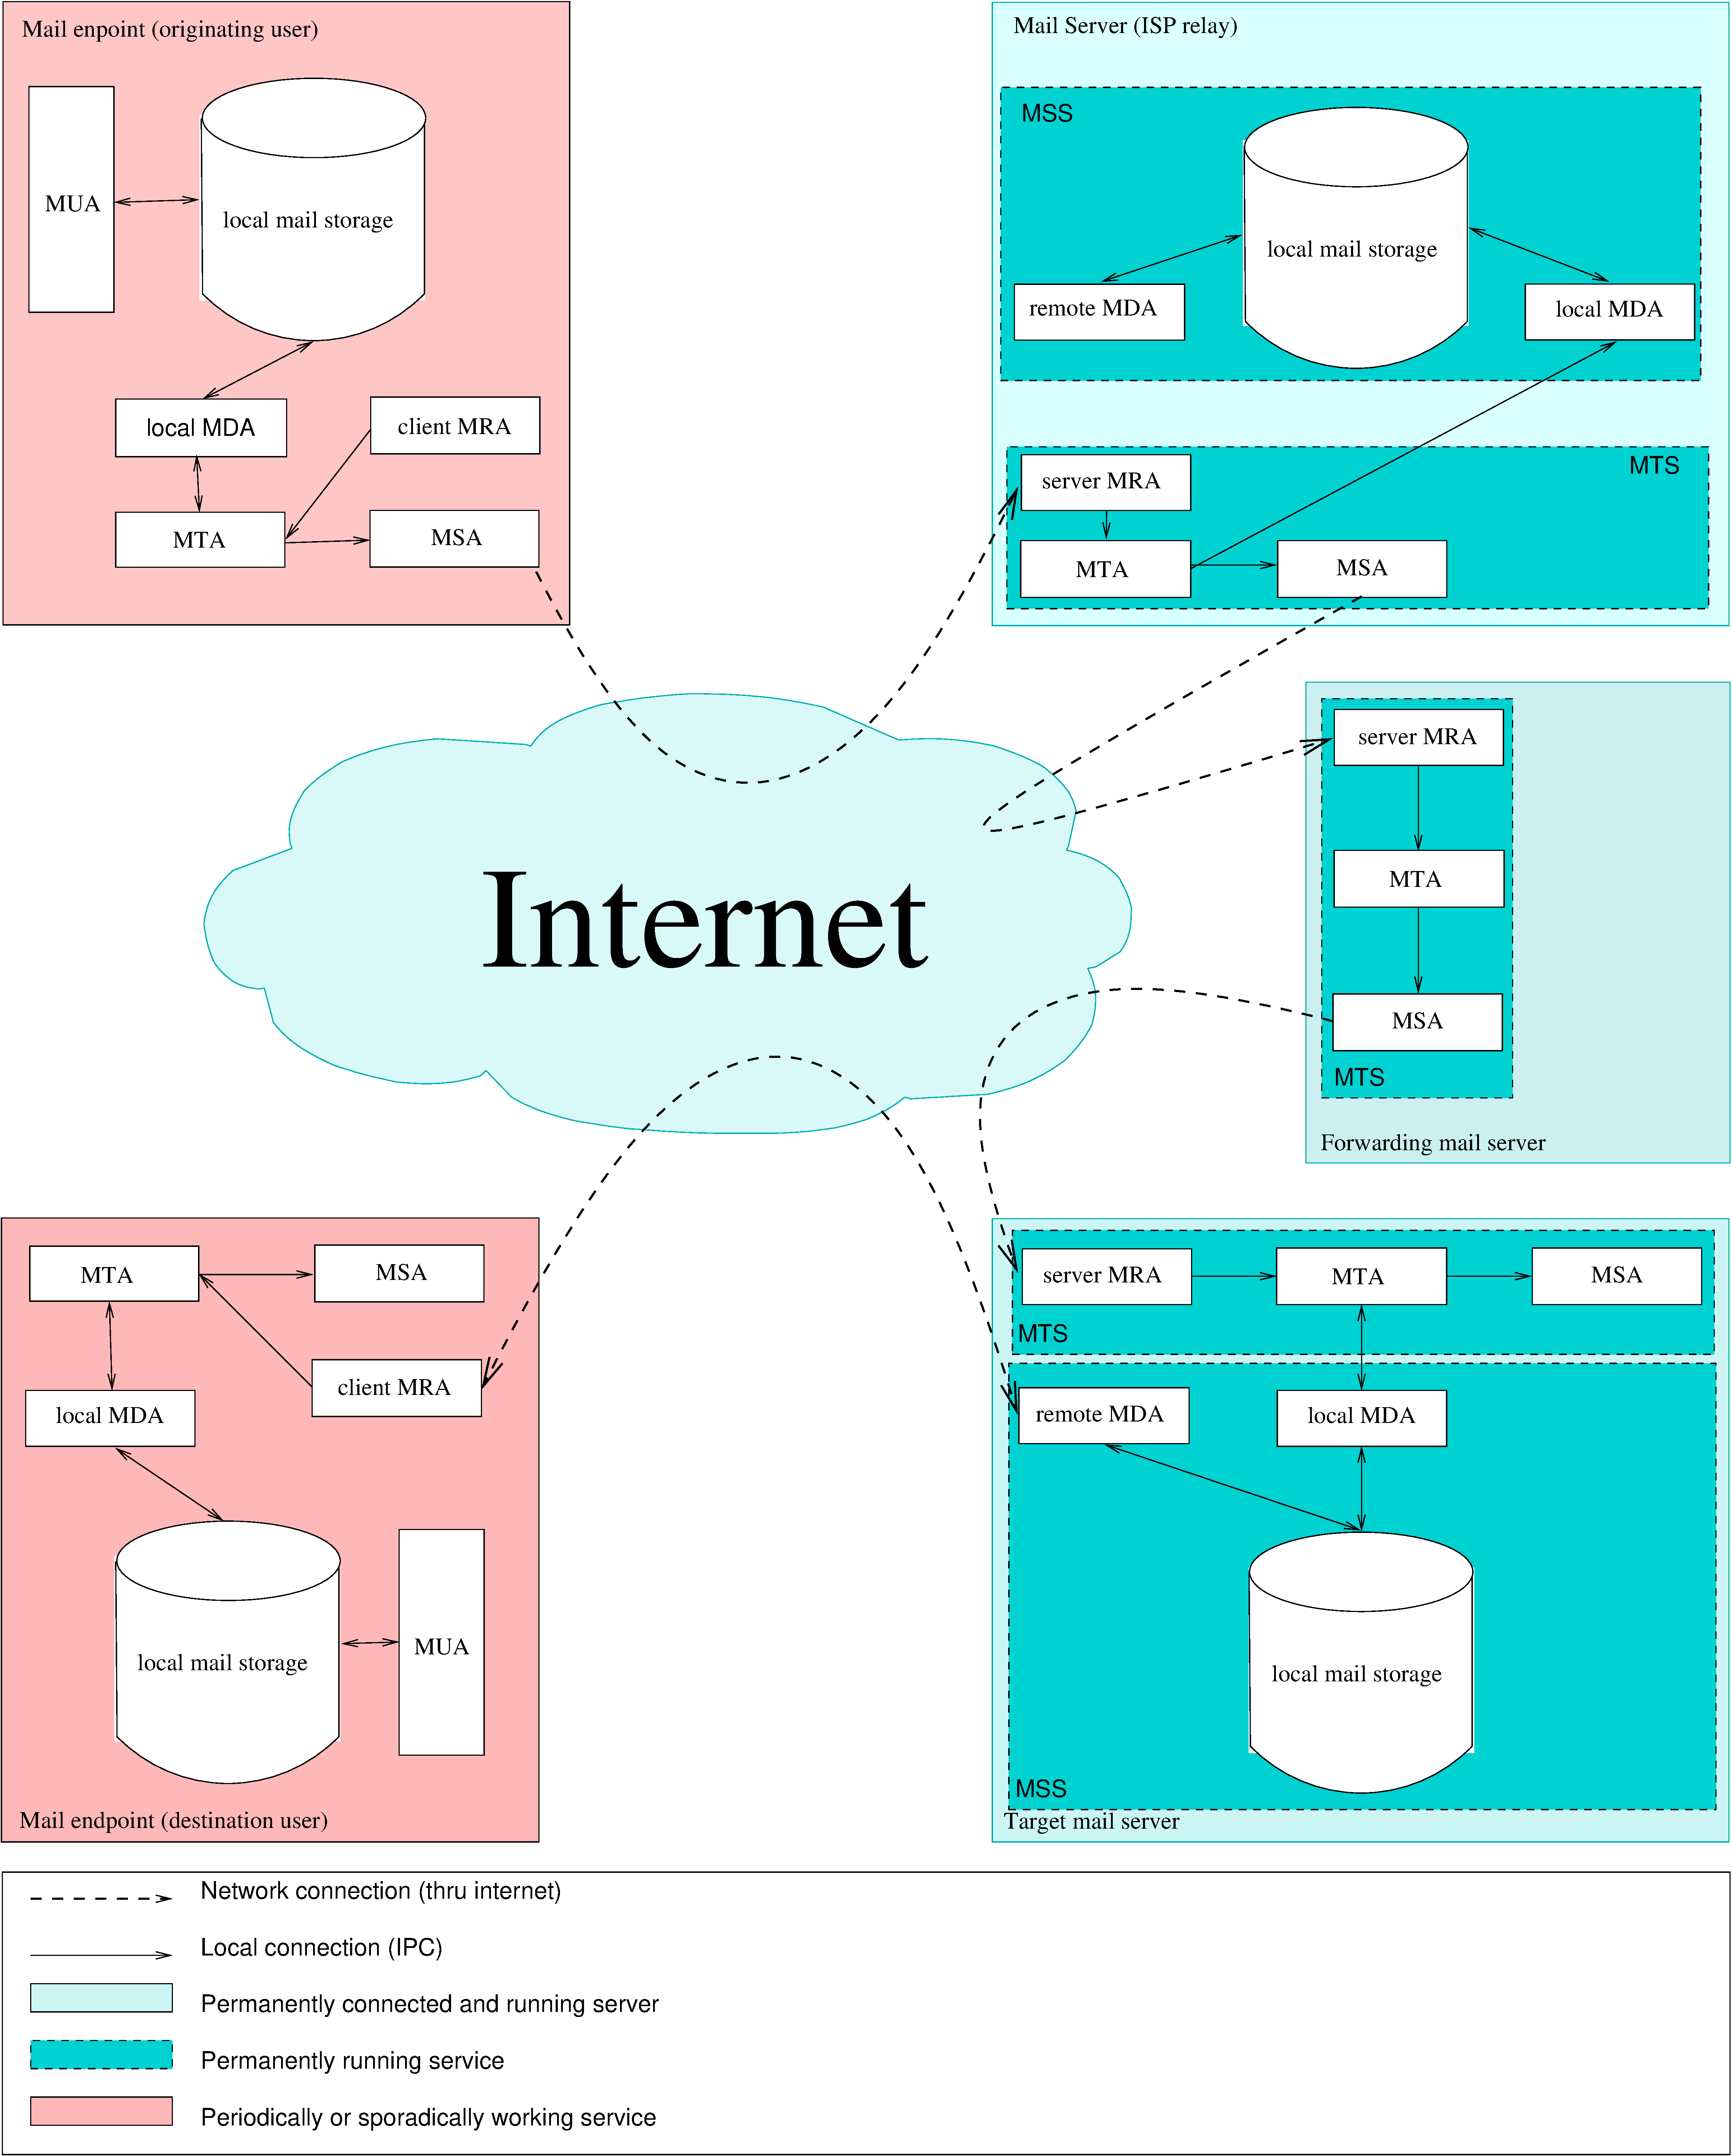
\includegraphics[width=\columnwidth]{inc/MailAgents1.pdf}
	\caption{Mail Agents}\label{fig:MailAgents}
\end{figure}

In the following paragraphs (for definitions) the term ``Mail'' is used synonymously to the term ``Message''. The reason why ``Mail'' has been chosen over ``Messages'' that a lot of terms do already exist in standard documents. In these documents the term mail is commonly used.\par

Mails are typically initiated by a Mail User Agent (\defref{MUA}). A MUA accesses a local mail storage which may be the server storage or a local copy. The local copy may be a cache only copy, the only existing storage (when mails are fetched and deleted from the server after retrieval) or a collected representation of multiple server storages (cache or authoritative).\par

Besides the MUA the only other component accessing a local mail storage is the Mail Delivery Agent (\defref{MDA}). An MDA is responsible for storing and fetching mails from the local mail storage. Mails destined for other accounts than the current one are forwarded to the MTA. Mails destined to a User are persistently stored  in the local mailstorage. It is important to understand that a mailstorage not nessesarily reflects a simple mailbox. It may as well represent multiple mailboxes (eg. a rich client serving multiple IMAP accounts) or a combined view of multiple accounts (eg. a rich client collecting mail from multiple \defref{POP} accounts. In the case of a rich client the local MDA is part of the software provided by the user agent. In the case of a mail server the local MDA is part of the local Mailstore (not necessarily of the mail transport service).

On the server side there are usually two components (services) at work. A ``Mail Transport Service'' (\defref{MTS}) responsible for mail transfers and a ``Mail Storage System'' which offers the possibility to store received Mails in a local, persistent store.\par

A MTS consists generally out of three parts. For incoming connects there is a daemon called Mail Receiving Agent (\defref{Server MRA}) is typically a \defref{SMTP} listening daemon. A Mail Transfer Agent (\defref{MTA}) which is responsible for routing, forwarding and rewriting mails. And a Mail Sending Agent (\defref{MSA}) which is responsible for transmitting mails reliably to another Server MRA (usually sent via \defref{SMTP}).\par

A MSS consists out of a local storage and delivery agents which do offer uniform interfaces to access the local store. They do also deal with replication issues and grant should take care of the atomicity of transactions committed to the storage. Typically there are two different kind of \defref{MDA}s. \defref{Local MDA}s offer possibilities to access the store via efficient (non network based) mechanisms (eg IPC or named sockets). This is usually done with a stripped down protocol (eg. \defref{LMTP}). For remote agents there a publicly -- network based -- agent available. Common Protocols for this \defref{Remote MDA}\ include \defref{POP}, \defref{IMAP}, or \defref{MS-OXMAPIHTTP}.\par

\subsection{Mail Endpoints}
\fxwarning{Move this section to appropriate location}
Mail endpoints consist typically of the following components:
\begin{itemize}
	\item A Mail User agent (\defref{MUA})
	\item A Local Mail storage (\defref{MUA})
	\item A Local Mail Delivery Agent (\defref{Local MDA})
	\item A Mail Transfer Agent (\defref{MTA})
	\item A Mail Sending Agent (\defref{MSA})
	\item A Mail Receiving Agent (\defref{MRA})
\end{itemize}

Only two of these components do have external interfaces. These are \defref{MSA} and \defref{MRA}. \defref{MSA} usually uses \defref{SMTP} as transport protocol. When doing so there are a couple of specialities. 
\begin{itemize}
	\item Portnumber is 587 (specified in \cite{RFC4409}).\\
	Allthough port numbers 25 and 465 are valid and do have usually the same capabilities, they are for mail routing between servers only. Mail endpoints should no longer use them.
	\item Connections are authenticated.\\
	Unlike a normal server-to-server (relay or final delivery) SMTP connections on port 25 clients should always be authenticated of some sort. This may be based on data provided by the user (eg. username/passsword or certificate) or data identifying the sending system (eg. IP address)\cite{RFC4409}. Failure in doing authentication may result in this port beeing misused as an sender for UBE.
\end{itemize}

Mail User Agents (MUA) are the terminal endpoint of a mail delivery. Mail user agents may be implemented as fat clients on a desktop or mobile system or as an interface over a different generic protocol such as HTTP (Web Clients). \par

Server located clients are a special breed of fat clients. These clients share the properties of fat clients except for the fact that they do not connect to the server. The client application itself has to be run on the server where the mail storage persists. This makes delivery and communication with the server different. Instead of interfacing with a MSA and a client MDA they may directly access the local mail storage on the server. On these systems the local mail storage may be implemented as a database in a user specific directory structure.

\subsubsection{Fat clients}
The majority of mail clients are fat clients. These clients score over the more centralistic organized web clients in the way that they may offer mail availability even if an internet connection is not available (through a client specific local mail storage). They furthermore provide the possibility to collect mails from multiple sources and store them in the local storage. Unlike Mail servers, clients are assumed to be not always online. In fact they may be offline most of the time. To guarantee the availability of a certain email address a responsible mail server for a specific address collects all mails (this is done by the \defref{MSS}) and provides a consolidated view onto the database when a client connects through a local or remote MDA.\par

As these clients vary strongly it is absolutely mandatory for the MDA that they are well specified. Lack in doing so would result in heavy interoperability problems. Most commonly the Protocols \defref{IMAP}, \defref{POP} and \defref{EWS} are being used these days. For mail delivery the SMTP protocol is used. \par

Fat clients are commonly used on mobile devices. According to  \cite{clientDistribution} in Aug 2012 the most common fat email client was Apple Mail client on iOS devices ($35.6\%$), followed by Outlook ($20.14\%$), and Apple Mail ($11\%$). \citetitle{clientDistribution2}\cite{clientDistribution2} as a more recent source lists in February 2014 iOS devices with $37\%$, followed by Outlook ($13\%$), and  Google Android ($9\%$).

\subsubsection{Server located clients}
server located clients build an absolute minority. This kind of clients have been used mainly in the days of centralized hosts. An example for a Server Located Client is the Unix command "`mail"'. This client reads a mail storage from a file in the users home directory.

\subsubsection{Web clients}
Web clients are these days a common alternative to fat clients. Most big provider companies use their own proprietary web client. According to \cite{clientDistribution2} the most common web clients are "`Gmail"', "`Outlook.com"', and "`Yahoo! Mail"'. All these Interfaces do not offer a kind of public plug-in interface. However,  they do offer IMAP-interfaces. This important for a future generalistic approach to the problem.

\subsection{Interfaces of Mail Endpoints}
There are two interfaces 

\fxwarning{add content here}

\subsection{S/MIME}
S/MIME is an extension to the MIME standard. The MIME standard allows in simple text oriented mails an alternate representation of the same content (e.g. as text and as html), or it allows to split a message into multiple parts which may be encoded. It is important to note that MIME encoding is only effective in the body part of a mail.

S/MIME as described in \cite{RFC3851} extends this standard with the possibility to encrypt mail content or to sign it. Practically this is achieved by either putting the encrypted part, or the signature into an attachment. It is important to know, that this method leaks significant parts of the data.

As the mail travels directly from sender to recipient both involved parties are revealed. Neither message subject nor message size or frequency are hidden. This method does offer limited protection when assuming an adversary with interest in the message content only. It does not protect from the kind of adversary in our case. 

The trust model is based on a centralistic approach involving generally trusted root certification authorities.

\subsection{PGP/MIME}
Exactly as S/MIME PGP\cite{RFC2440} builds upon the base of MIME. Although the trust model in PGP is peer based. The encryption technology does not significantly differ (as seen from the security model).

A good thing to learn from PGP is that there are peer based approaches offering limited possibilities for trust. The trust in PGP is based on the peer review of users. This peer review may give an idea of how well verified the key of a user is.

\fxwarning{add content here}

\subsection{XMMP}
\fxwarning{add content here}

\section{Proof of work}
Proof of work is one possibility to limit resource exhaustion on locally controlled resources. Traditional proofs are either CPU- or memory-bound. This means that they have to proof that they assigned a certain amount of their own CPU time or memory bandwidth to a problem posed by the receiving node.

In \cite{amiri2015theoretical} is a good summary of proposed proof of work methods. Although they are used there for the defence of DDoS-attacks (Distributed Denial of Service) they might as well be used for defence against misuse for UBE and (D)DoS of the Vortex system. The list has been shortened with irrelevant algorithms for this work and extended with newer research in that field.

In our case we are looking for a proof which imposes ideally the same amount of work to an attacker and a valid sender. Since an attacker need a lot more resources than a normal sender the amount of work should be for him unbearable. A normal sender on the other hand should be able to cover the load imposed by the system easily.

The website coinwarz and \cite{cryptomining-blog.com} list the current mining speeds on up to date hardware for several algorithms as shown in table \ref{tab:hashSpeed}.
\begin{table*}[t]
	\centering\tiny
	\begin{tabular}{|l|r|l|l|}\hline
		\diaghead{\theadfont Proof of work Criteria}{Proof of Work}{Criteria} 	 & \thead{Speed}	& \thead{hardness type} & \thead{Cryptocurrency} \\\hline
		Blake-256\cite{aumasson2008blake}   &  $11\, 200\, 000$ & FIXME          & Blakecoin\\
		CryptoNight                         &               $2$ & Memory or egalitarian & Monero\\
		EtHash\cite{ethash}                 &       $108\, 000$ & Memory and IO  & Ethereum, Ethereum-classic\\
		Equihash\cite{biryukov2016equihash} &               $1$ & FIXME          & Zclassic, Zcash\\
		Groestl\cite{gauravaram2009grostl}  &        $45\, 000$ & FIXME          & Groestlcoin, Diamond\\
		HEFTY1                              &           unknown & FIXME          & Heavycoin, Mjollnircoin \\
		Keccak\cite{bertoni2009keccak}      &   $1\, 000\, 000$ & FIXME          & Maxcoin, Startcoin, CryptoMeth\\
		Lyra2REv2    \cite{lyra2}           &        $30\, 000$ & Memory         & Vertcoin\\
		NeoScrypt                           &             $400$	& Memory         & Feathercoin, UFOCoin, OrbitCoin, Phoenixcoin\\
		\multirow{2}{*}{SHA-256} 	        &   $9\, 460\, 000$	& CPU            & UniversalCurrency, Mazacoin, Titcoin, Peercoin, Bitcoin, HAMRadioCoin, eMarl,        Digitalcoin-SHA-256, Zetacoin, Curecoin, Freicoin, \\
		                                    &                   &                & Tigercoin, Terracoin, Unbreakable, Myriadcoin-SHA-256, Joulecoin, Acoin, Tekcoin, Unobtanium, Namecoin, DevCoin, IxCoin\\    
		\multirow{3}{*}{Scrypt} 		    &       $110\, 000$	& Memory         & Einsteinium, Gulden, Casinocoin, Quatloo, GameCredits, DNotes, Auracoin, Novacoin, CHNCoin, Goldcoin, Florincoin, Megacoin, \\
		                                    &                   &                & Bottlecaps, Litecoin, Bitbar, DigiByte, Verge, Franko, BATA, Worldcoin, WildBeastBitcoin, BBQCoin, Nyancoin, Digitalcoin-Scrypt,  \\
		                                    &                   &                & Aricoin, Sexcoin, Spots, Emerald, Dodgecoin, Viacoin, Myriadcoin-Scrypt\\    
		Scrypt-Adaptive-NFactor             &           unknown & FIXME          & Vertcoin, Execoin, GPUcoin, ParallaxCoin, SiliconValleyCoin\\
		Scrypt-Jane                         &           unknown & FIXME          & YaCoin, Ultracoin, Velocitycoin\\
		Quark                               &        $20\, 000$ & FIXME          & MonetaryUnit, Quark, Securecoin\\
		X11                                 &        $34\, 400$	& FIXME          & Digitalcoin-X11, Dash, CanabisCoin, darkCoin, HiroCoin, X11Coin\\
		X13                                 &           unknown & FIXME          & MaruCoin, BoostCoin, X13Coin\\
		Yescrypt   \cite{yescrypt}          &           unknown & ROM-port       & Globalboost-Y \\
		\hline          
	\end{tabular}	
	\caption{comparison of of Proof of Work algorithms}
	\label{tab:hashSpeed}
\end{table*}

\subsection{CPU-Bound Proof of work}
CPU bound proof of work tries to assign a task to a request. By presenting a result the sender proofs that he solved a puzzle. Normally these puzzles may only be solved by brute force.

\subsubsection{Hash based puzzle by Juels and Brainard} 
The hash puzzle by \citeauthor{juels1999client} in \cite{juels1999client} works as follows: 
\begin{itemize}
	\item The requester requests an operation.
	\item The service provider sends a block of data back with a known number of missing bits at the end and a cryptographic hash of the original block (including the missing bits)
	\item The requester then brute forces the missing bits until he finds the correct bit sequence to complete the hash puzzle and sends it to the service provider.
\end{itemize}

This puzzle has several downsides. One of the biggest downsides is that the puzzle may be solved by using multiple instances in parallel. This allows a specialised adversary to build an efficient infrastructure for solving this kind of puzzle.

\subsubsection{Hash based puzzle by Aura, Nikander and Leiwo} 
The hash based puzzle by \citeauthor{aura2000resistant} in \cite{aura2000resistant} is an improved variant of \cite{juels1999client}. It works as follows:

\begin{itemize}
	\item The requester requests an operation.
	\item The service provider sends a nonce block $N_{sp}$ to the requester and a number $k$ (this number represents the difficulty).
	\item The requester chooses a nonce $N_{r}$.
	\item The requester brute forces  $puzzlesolution$ by solving $hash(identity_r, N_{sp}, N_{r}, puzzlesolution)=hashValueStartingWithKBitsOfZeroes$.
	\item The requester sends $N_r$ and $X$ it to the service provider.
\end{itemize}

The downsides of this puzzles are that it may be calculated in parallel. This allows a specialised adversary to build an efficient infrastructure for solving this kind of puzzle. Furthermore the client side nonce $N_r$ must be stored as long as the server side nonce $N_{sp}$ is not regenerated in order to avoid replay attacks.

\subsubsection{Modified Repeated Squaring Puzzle} 
\citeauthor{jeckmans2009practical} proposed in \cite{jeckmans2009practical} a Squaring hash puzzle. The algorithm is described as follows:

\begin{itemize}
	\item $Setup(\ell)$: the sever generates a new public parameter $sp$ with length $\ell$ bits using a (pseudo)random number generator. It then selects two random large primes $p$, $q$ and creates $n = p \times q$ out of this. The server also selects a difficulty for the puzzles, $k$. The algorithm then outputs $mk = 2^k  \mod \phi(n)$ and $\mathbf{params} = \langle k, sp, n \rangle$.
	\item $PuzzleGen(mk, req)$: $puz = \emptyset$ and $info = \emptyset$.	
	\item $PuzzleSol(puz)$: $g = H( \langle sp, id_C \rangle )$, $sol = g^{2^k} \mod n$.
	\item $PuzzleVer(info, mk, sol)$: This algorithm computes the generator, $g = H( \langle sp, id_C \rangle )$. The solution is then verified $sol \stackrel{?}{=} g^{2^k \mod \phi(n)} \mod n$.
	\item $BatchVer(info, mk, sol_i (1 \leq i \leq m))$: assume that the server has stored $m$ solutions to check, $sol_i$, 
	$1 \leq i \leq m$. Compute the corresponding generators $g_i = H( \langle sp, id_{C_i}\rangle )$, $1 \leq i \leq m$.  These solutions are then verified with batch verification using Equation $(\prod_{i=1}^{m}g_i)^{2^k} \mod n \stackrel{?}{=} \prod_{i=1}^{m} sol_i \mod n$.
\end{itemize}

This puzzle is a typical CPU bound puzzle compensating a lot of the drawbacks of \cite{aura2000resistant} and \cite{juels1999client} mentioned in the sections before. First it offers a potential verification in batches under the assumption that all solutions within the batch are correct. Secondly it is non-parallelizable. There is very little information to be stored on the server side and non of the information has a lifetime which is longer than the puzzle.


\subsubsection{Hinted Hash Puzzle} 
In \cite{1498523} the authors \citeauthor{1498523} proposed a protocol and is closely related to \cite{aura2000resistant}. The protocol itself is working as follows:

\begin{itemize}
	\item The requester requests an operation and includes a nonce $N_c$.
	\item The service provider sends a chosen puzzle $P$ and the hash answer $H(\langle A,N_s\rangle )$ to the requester.
	\item The requester brute forces $A$.
	\item The requester sends $A$ to the service provider.
\end{itemize}

In the original protocols hashes and nonces are resent in order to verify if the requests do still match the originally sent data. As they have no impacts on the mathematical side of the operation they have been eliminated in this description.

From today's view this protocol is however not very secure. Solutions may be searched in parallel and the protocol is susceptible to replay attacks as found result $A$ is replayed over the course of time to re-authenticate 

\subsubsection{Chained Hash Puzzle} 
\cite{groza2006} (CPU Bound)

\fxwarning{add content here}

\subsubsection{Targeted Hash Puzzle} 

\cite{4301429} (CPU Bound)

\fxwarning{add content here}

\subsubsection{Repeated Squaring Puzzle} 

\cite{rivest1996time} (CPU Bound)

\fxwarning{add content here}

\subsubsection{Discrete Logarithm Puzzle} 
The puzzle of \citeauthor{waters2004new} in \cite{waters2004new} are somewhat similar to a brute force attack in a DH key exchange. This puzzle is non-parallelizable and is related to the hint based puzzles.

\fxwarning{add content here}

\subsubsection{Subset sum puzzle} 

\cite{tritilanunt2007toward} (CPU bound)

\fxwarning{add content here}

\subsection{Memory-Bound Proof of work}
\subsubsection{Moderately hard, memory-bound functions} 

\cite{abadi2005moderately} (Memory hard)

\fxwarning{add content here}

\subsubsection{Memory bound puzzle based on pattern databases} 

\cite{doshi2006efficient} (Memory hard)

\fxwarning{add content here}

\subsubsection{Argon2}
\cite{biryukov2016argon2}

\fxwarning{add content here}

\subsubsection{Scrypt}
Scrypt was originally developed by \citeauthor{percival2009stronger} in \citeyear{percival2009stronger} and formally defined by \citeauthor{RFC7914} in \cite{RFC7914}. It was originally designed as a key derivation function for an online backup service called tarsnap. Acording to the tarsnap site (\href{http://www.tarsnap.com/scrypt.html}{http://www.tarsnap.com/scrypt.html}) the cryptocurrency Litecoin uses a simplified version of the scrypt as proof of work scheme.

\cite{forler2014memory}

\fxwarning{add content here}

\subsubsection{HashCash}
\cite{back2003hashcash}

\fxwarning{add content here}

\subsection{Summary for Proof of Work Algorithms}
\fxwarning{to check: Groza 2016 Cryptanalysis of an authentication protocol}

\cite{groza2005cryptanalysis}

\fxwarning{add Revisiting Difficulty Notions for Client Puzzles and DoS Resilience}

\cite{groza2012revisiting}

\fxwarning{check and possibly add}

\cite{tritilanunt2007toward}

\fxwarning{check and possibly add}

\cite{alwen2016efficiently}

\fxwarning{check and add}

\cite{dwork2003memory}

\fxwarning{check and possibly add}

\cite{cryptoeprint:2005:356}

\fxwarning{check and possibly add}

\cite{tromp2015cuckoo}

\fxwarning{add Merkle tree based Coelho, Fabien. "An (almost) constant-effort solution-verification proof-of-work protocol based on Merkle trees". Cryptology ePrint Archive, Report.}

\cite{coelho2008almost}

\fxwarning{check carefully; possibly bad}

\cite{abliz2009guided}
	
\fxwarning{add table from amiri2015theoretical here and extend with additional puzzles}

\fxwarning{isolated candidates: scrypt (memory hard) and sh-256 (cpu hard; beware of paralellisation)}

\section{Pseudo Random Number Generators \label{sec:prng}}
\fxwarning{add content here}

\fxwarning{refer to FC 1750: Randomness Recommendations for Security}


\section{Known Attacks}
In the following sections we emphasize on possible attacks to an anonymity preserving protocols. In the following sections we describe classes of attacks. These attacks may be used to attack the anonymity of any entity involved in the message channel. In a later stage we test the protocol for immunity against these classes of attacks.

\subsection{Broken Encryption Algorithms}
Encryption algorithms may become broken at any time. This either to new findings in attacking them, by more resources being available to an adversary, or by new technologies allowing new kind of attacks. A good protocol must be able to react to such threads in a timely manor. This reaction should not rely on a required update of the infrastructure. The grade of security should solely be controlled by the users. 

We cannot do a lot for attacks of this kind to happen. However -- we might introduce a choice of algorithms and key sizes to give the user a choice in the degree of security he wants to have.

\subsection{Attacks Targeting Anonymity}
All attacks targeting users anonymity is a main focus of this work. Many informations may be leaked and the main goal should therefore rely on the principles established in security.

\begin{itemize}
\item Prevent an attack\\
      This can only be done for attacks which are already known and may not be realistic in all cases. In our protocol we have strict boundaries defined. A node under attack should at any time of a valid protocol usage (this excepts bandwidth depletion attacks) be able to block malicious identities. Since establishing new identities is costly an attacker should always require far more resources than the defender.
\item Minimize attack surface\\
      This part of the attack prevention is included by design in the protocol.
\item Redirect an attack\\
	  Although this is not done by the implementation it is possible to handle suspected malicious nodes differently.
\item Control damage\\
      For us this means leaving as little information about identities or meta information as possible on untrusted infrastructures. If we leave traces (i.e. message flows, or accounting information) they should have the least possible information content and should expire within a reasonable amount of time.
\item Discover an attack\\
      The protocol is designed in such a way that discovering attacks (such as a query attack) may be done. However -- we consider active attacks just as part of the ordinary message flow as an immediate result. 
\item Recover from an attack\\
      An attack does always impose a load onto a systems resources regardless of its success. It is important that a system recovers almost immediately from an attack and is not covered in a non or only partial functional state either temporarily or permanently.
\end{itemize}

In the following subsections we list a couple of attack classes which have been used against systems listed in \ref{sec:sysImpl} or the respective academic works. We list the counter measures which have been taken to deflect these attacks.

\subsubsection{Probing Attacks}
Identifying a node by probingand check their reaction is commonly done when fingerprinting a service. As a node is participating in a network and relaying messages probing may not be evaded. However, it may be made costly for an adversary to do systematic probing. This should be taken into account. 

One strategy to avoid would be to put high costs onto clear text requests in such a way that a clear text request may have a long reply time (e.g. up to one day). An early retry of the same identity would lead to automatic blacklisting. This is however an insufficient strategy as a huge adversary may have lots identities in stock. Requesting a particularly long key as an plain text identity does not make sense either as these as well may be kept in stock. We may however force a plaintext request to have a hash following certain rules. We may for example put in a requirement that the first four bytes of the hash of a header block translates to the first four characters of the receiving address


\fxwarning{add content here; Reduce attractiveness of cleartext probing attacks by discard 80\% of messages and blacklist on early retry?}

\subsubsection{Hotspot Attacks}
\fxwarning{add content here}

\subsubsection{Message Tagging and Tracing}
\fxwarning{add content here}

\subsubsection{Side Channel Attacks}
\fxwarning{add content here}

\subsubsection{Timing Attacks}
\fxwarning{add content here}

\subsubsection{Sizing Attacks}
\fxwarning{add content here}

\subsubsection{Bugging Attacks}
Numerous attacks are available through bugging of a protocol. In this chapter we outline some of the possibilities and how they may be countered:

\paragraph{Bugging through certificate or identity lookup:} Almost all kind of proof of identities, such as certificates, offer some kind of revocation facility. While this is a perfect desirable property of these infrastructures they offer a flaw. Since the location of this revocation information is typically embedded in the proof of identity an evil attacker might use a falsified proof of identity with a recording revocation point.
	      
There are multiple possibilities to counter such an attack. The easiest one is to do no verification at all. This is however not desirable from the security point of view. 

Another possibility is to only verify trusted proof of identities. By doing so the only attacker could be someone having access to a trusted source of proof of identities. 

A third possibility is to relay the request to an other host either by using an anonymity structure such as Tor or by using its own infrastructure. Using Tor would violate the ``Zero Trust'' principle we are aiming for. Furthermore this measure would only conceal the source of the verification. It would not hide the fact that the message is being processed. 

A fourth and most promising technology would be to force the sender of the certificate to include a ``proof of non revocation''. This could be a timestamped and signed partial CRL. Such a mandatory proof of non-revocation would allow a node to verify the validity of a certificate without being forced to disclose itself by doing a verification. On the downside has to be mentioned that including a proof of non-revocation involves the requirement to accept a certain amount of caching time to be accepted. This allowed caching time reduces the value of the proof as it may be expired in the mean time. It is recommended to keep the maximum cache time as low as 1d in order to avoid that revoked certificates may be used. 

\paragraph{Bugging through DNS traffic:} A widely common protocol in the internet is DNS. Almost all network related programs use it without thinking. Normally is the usage of such a protocol not a minor issue since the resolution of a lookup usually done by an ISP. In the case of a small ISP this might however already become a problem.

The bugging in general attack works as follows: We include a unique DNS name to be resolved by a recipient. This can be done most easily by including an external resource such as an image. A recipient will process this resource and might therefore deliver information about the frequency of reading, or the type of client. 

It must be taken into account that the transport layer will always do DNS lookups and that we may not avoid this attack completely. We may however minimise the possibilities of this attack.

\paragraph{Bugging through external resources:} An easy attack is always to include external resources into a message and wait until they are fetched. In order to avoid this kind of attack plain text or other self contained formats should be used when sending a message. As we may not govern the type of contained message we can make at least recomendations concering its structure

\subsection{Denial of Service Attacks}
\subsubsection{Censorship}
Where as traditional censorship is widely regarded as selective information filtering and alteration a very repressive censorship can even include denial of information flows in general. Any anonymity system not offering the possibility to hide in legitimate information flows is therefore not censorship resistant.

\subsubsection{Credibility Attack}
Another type of DoS attack is the credibility attack. While not necessarily a technical attack it is very effective. A system not having a sufficiently big user base is offering thus a bad level of anonymity due to the fact that the anonymity set is too small or the traffic concealing message flow is insufficient. 

In a credibility attack a systems reputation is degraded in such a way that the system is no longer used. This may be achieved in serveral ways. This is usually done by reducing the reputation of a system.

This may be achieved in several ways. Examples:
\begin{itemize}
	\item Disrupt functionality of a system.\\ 
	This may be done by blocking ports the messaging protocol uses or blocking selectively messages. It may be done by removing publicly known participants from the internet either by law or by threatening.
	\item Publicly dispute the effectiveness of a system.\\
	This is a very effective way to destroy a system. People are not willing to use a system which is compromised if the main goal of using the system is avoiding being observed.
	\item Reduce the effectiveness of a system.\\
	A system may be considerably being loaded by an adversary to decrease the positive reception of the system. He may further use the system to send UBE to reduce the overall experience when using the system. Another way of reducing the effectiveness is to misuse the system for bad purposes and making them public.
	\item Dispute the credibility of the system founders.\\
	Another way of reducing credibility of a system is to undermine its creators. If -- for example -- people believe that a founders interest was to create a honey pot (e.g. because he is working for a potential state sponsored adversary) for personal secrets they will not be willing to use it.
	\item Dispute the credibility of the infrastructure.\\
	If an infrastructure is known or suspected to be run by a potential adversary peoples willingness to believe into such a system might be drastically reduced.
\end{itemize}

\chapter{Applied Methodes\label{sec:appliedMethods}}
Based in the findings of the previous chapter we used the following methodology in order to find a solution:
\begin{enumerate}
	\item Identify problem hotspots for a new protocol.
	\item Design a protocol which addresses the previously identified hotspots.
	\item Build a protocol prototype.
	\item Analyse the protocol for weaknesses using attack schemes.
	\begin{enumerate}
		\item Tagging/Bugging attacks
		\item Tracing attacks
	\end{enumerate}
\end{enumerate}

\section{Problem Hotspots}
Starting off from the previous research we identified several hotspots which have to be taken care off. The following sections list identified problems and the possible countermeasures which have not been broken in the past.

\fxwarning{add content here}

\subsection{Zero Trust Philosophy}
One main disadvantage of almost any system listed in section \ref{sec:sysImpl} is that a trust (unlimited or limited) has been put into the infrastructure. In example when using Tor you need to trust the directory servers. Control over the directory servers might give an attacker the possibility to redirect a connection to controlled entry and exit nodes which would then break anonymity. In general control of entry and exit nodes makes a system vulnerable. 

To avoid this problem we decided to apply a zero trust model. We do not trust any platform except for the sending and receiving computer. We assume that all other devices are compromised and do create detailed logs about what they are doing. We furthermore assume that traffic on the network layer is observed and recorded at any time. This philosophy creates very hard to meet goals. But by assuming so we prevent the system from leaking information through side channels.

\begin{requirement}{zeroTrust}{Zero Trust}
	No infrastructure should be trusted unless it is the senders or the recipients infrastructure.
\end{requirement}	

\subsection{Information leakage}
Information of messages or their meta data should not be leaked. This means that in a normal message flow any hop should be a valid sender, a valid recipient, or a valid mix this implies some kind of peer-to-peer (P2P) design. 

\subsubsection{P2P design}
A main problem of the P2P design is that usually port forwarding or a central infrastructure is required. Technologies such as ``hole punching'' and ``hairpin translation'' usually require central infrastructures to support at least the connection and may be depending on the client infrastructure being used fragile or ineffective. To avoid these problems we decided to rely on traditional centralistic transport infrastructures. As the proof of concept we decided to use SMTP. 

The approach supports however even mixing transport media. This makes it harder for an attacker to trace a message as the message flow may go through any suitable transport protocol at any time of message transfer.

\begin{requirement}{P2P}{P2P}
	Mixes and peers must be undistinguishable.
\end{requirement}

\subsubsection{Decoy traffic generation}
In order to create decoy traffic in an untrusted way we need means to increase an decrease messages in size without knowledge of the routing node. An easy approach would be to create decoy traffic in the initial message. This would however create a pattern of decreasing message size in the net. To avoid this we introduced a set of operations to be applied to the original message. The operations are done in such a way that a mixer is unable to tell whether the message size or decrease results in decoy traffic generation/removal or not.

The main message operations are:
\begin{itemize}
	\item Split a message in two parts.
	\item Merge two messages.
	\item Fork off a block xor'ed (create a new random block of the received message size, then use a bitwise xor of these blocks to create a new block. Send any or all of these blocks further).
	\item Join two blocks xor'ed (take two blocks and xor them together)
\end{itemize}

At this point we could have used homomorphic encryption instead of xor. This would however add a lot of complexity to the algorithm with no obvious gain. The bitwise xor however allows a cheap fast operation and it allows to split and join information at will. Furthermore the implications of this operation are well known and researched.

\subsubsection{Message tagging or bugging protection}
It is important to the protocol that any operation at any point of the protocol handling which is not foreseen should result in the failure of message transport. This makes the protocol very fragile but it prevents mixes from introducing tags which may be followed throughout the system.

In our approach we give a single mix the full control over the message hiding/blending layer. This means that every mix decides for the content there. However -- This data is ephemeral and will (or may) be removed in the next node. The data received by a mix may be used to generate a ``pseudo reply'' on the blending layer to transport any other message (related or unrelated) back to the sending node. So tagging on this layer is worthless.

The reason for not giving control over the behaviour to this layer to the sender of the message is simple. By giving him control over it we would allow him to use the information provided here as the main medium. As an immediate result the system would suitable to blackmail any user of the world. It furthermore would create unintentional ``exit nodes'' to the system which might oppose further legal threads for participants.

\begin{requirement}{untagable}{untagable}
	The message should be untagable (neither by a sender, or by an intermediate party such as a mixer).
\end{requirement}

\begin{requirement}{unbugable}{unbugable}
	The message should be unbugable (neither by a sender, or by an intermediate party such as a mixer).
\end{requirement}

\subsubsection{Message replay protection}
Message reply protection is crucial for such a system. With the ability to replay a message an adversary may ``highlight'' a message flow as it would always generate the same traffic pattern. So there needs to be a reply pattern protecting the protocol from message replay. As we do have MURBs in our protocol this is a problem. A MURB is by design replayable. We therefore need a possibility for the original sender using a MURB to make messages distinguishable which may not be used by an adversary.

\begin{requirement}{replay}{replay}
	A message must not be replayable
\end{requirement}

It should be able to increase and shrink in size or all messages must have uniform size. Decoy traffic should not be distinguishable from true message traffic. 

\subsubsection{No Dedicated Infrastructure Philosophy}
There should be no infrastructure dedicated for the operation of the solution. This avoids single point of failures as well as the possibility for an adversary to shut down this infrastructure to disrupt the operation of the system as a whole. This requirement is already covered implicitely in \ref{req:zeroTrust}.

\subsection{Accounting}
The infrastructure must not be misused as UBE sending infrastructure. This implies that sending messages is connected to some kind of ``cost''. ``Costs'' must be connected to some kind of identity to allow accounting. Linking to a a global identity would allow to assign traffic to a real world user. Therefore the protocol must allow to create ephemeral local identities not linked to a real identity.

\begin{requirement}{accounting}{accounting}
	The system must be able to do accounting without being linked to a real identity.
\end{requirement}

\subsection{Anonymisation}
The system must allow to anonymise message source and message destination at any point. It should not be visible to the infrastructure protocol whether a message has reached its destination or not. 

\begin{requirement}{anon}{anonymisation}
	System must be able to anonymise sender and recipient at any point of the transport layer and at any point of mixing unless it is the sender or the recipient itself.
\end{requirement}

\subsection{Initial Bootstraping}
The system must allow to boot strap from a zero knowledge or near zero knowledge point. Starting off from this point the protocol must be able to extend the network on its own.

\begin{requirement}{boot}{bootstrapping}
	The system must allow to boot strap from a zero knowledge or near zero knowledge point and extend the network on its own. 
\end{requirement}

\subsection{Cypher selection}
In This Protocol a lot of encryption and hashing algorithms have to be used. This Choice should be explained. 

From the requirements side we have to follow the following principle:
\begin{requirement}{cryptVar}{encryption variety}
	The system must be able to use multiple symmetric, asymmetric, and hashing algorithms in order to immediately fall back to a secure algorithm for all new messages if required. 
\end{requirement}

First of all we need a subset of encryption algorithms all implementations may rely on. Defining such a subset guarantees interoperability between all nodes regardless of their origins. 

Secondly we need to have a spectrum of algorithm in such a manor that it may be (a) enlarged if necesary and (b) there is an alternative if an algorithm (or a mathmatical problem class) is broken (so that algorithms may be withdrawn if required without affecting the function in general). 

And third due to the onion like design described in this document asymmetric encryption should be avoided in favour of symmetric encryption to minimize losses due to the key length and the generally higher CPU load opposed by asymmetric keys.

If the algorithm is generally bound to specific key sizes (due to S-Boxes or similar constructs) the key size is incorporated into the definition. If not the key size is handled as parameter.

The key sizes have been chosen in such a manor that the key types form tuples of approximately equal strength. The support of Camelia192 and Aes192 has been defined as optional. But as they are wildly common in implementations they have already been standardized as they  build a possibility to step up security in future.

Having these criteria for choice we chose to use the following keys and key sizes:
\begin{itemize}
	\item Symetric
	\begin{itemize}
		\item AES (key size: 128, 192, 256)
		\item Camellia (key size: 128, 192, 256)
	\end{itemize}
	\item Asymetric
	\begin{itemize}
		\item RSA (key size: 2048, 4096, 8192)
		\item Named Elliptic Curves
		\begin{itemize}
			\item secp384r1
			\item sect409k1
			\item secp521r1
		\end{itemize}
	\end{itemize}
	\item Hashing
	\begin{itemize}
		\item sha384
		\item sha512
		\item tiger192
	\end{itemize}
\end{itemize}

Within the implementation we assigned algorithms to a security strength level:
\begin{itemize}
	\item LOW\\
	      AES128, RSA1024
	\item MEDIUM\\
	      AES192, RSA2048, ECC secp384r1
	\item HIGH\\
		  RSA4096, ECC sect409k1, sha384
	\item QUANTUM\\
	      AES256, RSA8192, ECC secp521r1, sha512
\end{itemize}

This allows to categorize the used algorithms to a strength. This list however should only serve the purpose of selecting algorithms for people without cryptological know how.

\fxwarning{Fix content (copied from first version). Be careful here!}

\subsection{Reed-Solomon function}
\fxwarning{add content here}

\subsection{Usability}
The system must be usable without cryptographic know-how and with well known tools. This is necessary to accept the system broadly and makes it easy to use for peoples already communicating.

\begin{requirement}{easy}{easy handleable}
	The system must be usable without cryptographic know-how and with well known tools.
\end{requirement}

\section{Protocol outline}
The protocol itself is independently from the transport layer specified. We emphasize in this section to the general building blocks, the cryptographic structure, and the general protocol attributes. In section \ref{sec:spec} we will then further elaborate the protocols inner structure.

The protocol is built on multiple layers. On the logic side the protocol is split into two parts:
\begin{enumerate}
	\item Transport Layer\\
	      This Layer is provided by normal internet infrastructures. The main goal is to hide or blend our protocol into ordinary traffic within that layer.
	\item Blending and subsequent layers\\
	      These layers may be provided by any user of the internet. Since these layers may be mixes only or valid endpoints they may or may not be publicly known. In a first implementation we build this system as a normal Java application. The main goal is to compile afterwards either native code and run it on a SoC like infrastructure such as a RaspberryPi or port it to an android device.
	      
	      We may further split these layers into
	      \begin{enumerate}
	      	\item Blending layer\\
	      	      This layer takes messages and creates transport layer conformant messages. In an ideal case the messages generated by this layer are undistinguishable from the normal message traffic and the embedded message is only visible for the receiving node.
	      	\item Routing layer\\
	      	      The routing layer disassembles and reassembles messages. This operation guarantees that messages are generated in such a way that decoy traffic is not differentiable from non decoy traffic.
	      	\item Accounting layer\\
	      	      The accounting layer has three jobs. First he has to authorise the message processing after decrypting the header block. Secondly he handles all header request blocks and the reply blocks. And third, it keeps track of the accounting in regard to the sent messages.    
	      \end{enumerate}
\end{enumerate}

\subsection{Protocol Terminology}

\begin{itemize}
	\item \textbf{Sender:} The user or process originally composing the message.
	\item \textbf{Recipient:} The user or process destined to receive the message in the end.
	\item \textbf{Mix:} Any node processing the message. Please note all nodes are mixes.
	\item \textbf{Message:} The ``real content'' to be transferred from the sender to the recipient
	\item \textbf{Payload:} Any data transported between mixes regardless of the meaningfulness or relevance to the message.
	\item \textbf{Decoy traffic:} Any data transported between mixes which has no relevance to the message at the final destination.
	\item \textbf{Identity:} A tuple of a routable address, and a public key.
	\item \textbf{Ephemeral Identity:} An identity created on any node with a limited lifetime anyone possessing the private key (proven by encrypting with it) is accepted as representative of that identity.
\end{itemize}


\fxwarning{add more}

\subsection{Vortex Communication model}
In this section we introduce a new consistent, transport independent model for representing the different protocols used by Vortex.

\fxwarning{add more}

\subsection{Transport Layer}
For our test we used a custom transport layer allowing us to monitor all traffic easily, and build structures in a very flexible way. This can be done with a minimum amount of work for setup  and deployment. It furthermore works across multiple hosts in a broadcast domain. The API may be used to support almost any kind of transport layer.

We identified in the previous section the following protocols as suitable for transport:
\begin{itemize}
	\item SMTP
	\item XMPP
\end{itemize}

For a prototype we will implement a SMTP-Transport agent.

\subsection{Blending Layer}
The blending layer is taking care of multiple problems:
\begin{itemize}
	\item It is translating the message block into a suitable format for transport\\
	      This includes jobs such as embedding a block as encoded text, as a binary attachment, or hide it within am message using steganography.
	\item Extract incomming blocks\\
	      Identify incomming messages containing a possible block and extract it from the message.
	\item Do housekeeping on the storage layer of the transport protocol\\
	      It may be required that messages are deleted from time to time in order to stay below sizing quotas of an account.      
\end{itemize}

We define the blending layer to work as follows when receiving messages:

\begin{enumerate}
	\item Log arrival time (in UTC) on the transport layer.
	\item Extract possible blocks.
	\item Apply decryption on a suspected header block .
	\item Identify header block as valid by querying the accounting.
	\item Extract and decrypt subsequent blocks.
	\item Pass extracted blocks and information to the routing layer.
\end{enumerate}

We define the blending layer to work as follows for sending messages:

\begin{enumerate}
	\item Assemble message as passed on by the routing layer.
	\item Using the blending method specified in the routing block build an empty message. 
	\item Create a message decoy content.
	\item Send the Message to the appropriate recipient using the transport layer protocol.
\end{enumerate}

There is no specification on the housekeeping part of the blending layer as this part is specific to the requirements of the account owner. We do however recommend to handle messages exactly as if the messages would be handled on a account handled by a human. 

\subsection{Routing Layer}
The routing layer receives the message blocks in a decrypted and authorised form from the blending layer. and processes them as follows:

\begin{itemize}
	\item Build structure representing the block building and the appropriate block IDs.
	\item Schedule all Routing blocks for processing in an priority queue.
	\item Authorise all routing blocks ready for processing with the calculated block sizes.
	\item Process blocks.
	\item Send prepared building blocks to the Blending layer.
\end{itemize}

\subsubsection{Block Structure}
The main block structure is defined as a sequence of blocks.

The block sequence starts with a header containing a symmetric key encrypted with public key of the current node and a header block containing the immediate details to decrypt the subsequent blocks (if any).

The header block is followed by a routing block. This block contains information required for subsequent routing. According to this block currently valid data blocks may be assembled and sent to a different location. 

The next block is the routing log block. This block protocols the routing information of a message and is somewhat similar to an onionized variant of the received headers in SMTP.

The final sequence of blocks are data blocks. They contain the actual data or decoy traffic.

\subsubsection{MURBs\label{sec:murb}}
The protocol allows to use MURBs. This enables a user to send a limited amount of times a message to an anonymous receiver without having any knowledge about its name or the location or infrastructure he is using.

A MURB in our term is a completely prepared routing instruction built by the recipient of a message. The sender has only the routing blocks and the instructions to assemble the initial message. It has no knowledge about the message path except for the first message hops.

As a MURB is a routing block it generates the same pattern on the network each time it is used. In order to avoid statistical visibility we need to limit the number of uses per MURB. As a maximum number of usages the number 127 has been chosen. This number allows to be used for automated messages. A minute pattern would disappear latest after 2 hours and an hourly pattern after 5 days.

\fxwarning{add something about murbs and the dangers of expiring quotas}

\section{Protocol design}
In this section we emphasize on the protocol blocks. These blocks are extracted from the blending layer and passed to the routing layer. A Vortex message is split into two main parts. The header block and the main block. The header block is divided into the two sub parts ``headerKey'' and ``identity block''. Although those blocks are described in \ref{app:rfcMessageVortexMainpp} as ASN.1 encoded structures they are not. In the message they are length prefixed fields.

In reality the structure is as follows:
\begin{itemize}
	\item headerKey size as 16 bit unsigned int (big endian)
	\item headerKey bytes
	\item identityBlock size as 16 bit unsigned int (big endian)
	\item identityBlock bytes
	\item mainBlock size as 32 bit unsigned int (big endian)
	\item mainBlock bytes
\end{itemize}
The reason for not using ASN.1 encoding is that it might be possible to identify the unencrypted message on the transport layer as vortex message due to the ASN.1 structure. By switching to a length prefixed structure we make it impossible for an adversary to identify the unencrypted structures of a vortex message.

\fxwarning{replace with image}


\subsection{Header block}
The header block contains the identity and should contain all information required to decide whether subsequent blocks of the message should be handled.

The header block contains the following data:
\begin{itemize}
	\item A symmetric header key (header key)\\
	      This key is encrypted with the receiving identities public key. This key guarantees an efficient handling of the header data. As the number of bytes in the header is limited a receiving node may assign all subsequent work to a known identity or discard it.
	\item An identity block (identityBlock)\\
		  This block contains a number of data which reflects the identity of the sender and the use of this (and subsequent blocks).
		  \begin{itemize}
		  	\item sending ephemeral identity public key (identityKey)
		  	\item serial
		  	\item maximum number of replays for the serial for this identity
		  	\item Minimum number of seconds for replay protection.
		  	\item validity period for this block (in seconds)
		  	\item Symmetric decryption key for subsequent blocks
		  	\item Chain secret for the forwarding block\\
		  	      If specified the specified secret should be named in all subsequent blocks.
		  	\item Protocol requests to this node
		  	\item Identifier and padding for proof of work
		  \end{itemize}
	\item An identity signature (identitySignature)\\
	      Contains a signed hash (hash type is specified in identityBlock.hash) with the senders private key.
\end{itemize}

\subsubsection{Ephemeral Identity}
The identity in this header block is an ephemeral identity. It exists for a limited amount of time (recommended <90d). Creating a new ephemeral identity is done with an identity request. This identity is mapped to all accounting figures.

\subsubsection{Requests\label{sec:request}}
Requests are always embedded in a header block. All requests are answered with a provided MURB (which is recommended to have a maximum replay value of 1).

There are several header requests defined:

\paragraph{newIdentity request:} This request may be answered with either a reject or a puzzle which is required to solve. Solving the puzzle results in the creation of the identity on the node. Identities may be rejected by the node for various reasons:

\begin{itemize}
	\item The node is not accepting newIdentity requests
	\item The identity is already taken.
	\item The identity is not strong enough (should be a longer key).
	\item The used encryption scheme is not supported by the node.
\end{itemize}

An identity may be rejected if the wrong types of keys and key sizes are used. However it must accept at least the key types and sizes it uses for its own identity.

If an identity is rejected the request may not be replayed by the same identity again. A sending party must generate a new identity for a new request. 

This request should be by far the most expensive request. It must at any time be more expensive to request a new identity compared to raise the quota of an existing one.

An identity is always ephemeral and expires after a given period of time. An identity may not be prolonged for security reasons. This oposes problems when using reply blocks. a reply block can only be valid as long as all included identities are valid. To counter this weakness without weakening security a ctxlessNewIdentity block may be sent to a reply block owner providing him with a new reply block.

\paragraph{queryPeer request:} A peer request is a request for publicly known Vortex nodes. This request does offer the possibillity of harvesting the Vortex network. To counter this the following limitations should apply:
\begin{itemize}
	\item The request should be very costly
	\item Only nodes avertising themselves as public are disclosed.
	\item Only one or two nodes should be disclosed upon request.
	\item The number of requests should be limited per identity.
	\item A node should always pick random nodes out of a 5\% pool of known Vortex addresses.
\end{itemize}

These measures limit the effectivity of harvesting attacks while giving a normal node the possibility of bootstrapping itself.

\paragraph{queryCapabillity request:} This request is the only request answered as a clear text request. To minimize probing possibilities this request should be only answered if the node owner agrees or generally by public nodes.

\paragraph{messageQuota request:} This request raises the number of routing blocks which may be processed for an identity. A node may reject this request depending on the load of the node, personal preferences, or because this identity causes too much traffic.

It is normally answered for all valid identities only. The node may answer it for recently expired identities. It is however not recommended to send a reply to an unknown identity as this behaviour might be used for probing of a node.

\paragraph{transferQuota request:} This request raises the number of bytes which may be transferred for an identity. A node may reject this request depending on the load of the node, personal preferences, or because this identity causes too much traffic.

It is normally answered for all valid identities only. The node may answer it for recently expired identities. It is however not recommended to send a reply to an unknown identity as this behaviour might be used for probing of a node.

\paragraph{queryQuota request:} This request instructs the node to send information about the given identity.

It is normally answered for all valid identities only. The node may answer it for recently expired identities. It is however not recommended to send a reply to an unknown identity as this behaviour might be used for probing of a node.

\subsubsection{Replys to Clear Text Requests}
It is up to the decision of the node whether it wants to answer a clear text request or not. Recommended for this behaviour is to discard plain text requests. 

This should only be a problem when bootstrapping or when adding new identities to the own address book. 

\subsection{Main block}
The main two block types are routing blocks and payload blocks. 

Routing blocks contain an onionised route chosen by the builder of the routing blocks and may contain instructions for building a message.

Payload blocks contain an encrypted message, parts of it or simply decoy traffic.

\subsubsection{Routing Blocks}
Routing blocks contain the following information:
\begin{itemize}
	\item The node specification of the next hop (requires a full identity; may be not there if no next hop)
	\item Purpose of routing block (May be normal/statusOK/statusError)
	\item The moment of processing as a range in seconds since the time of arrival.
	\item Retention time in seconds since the time of arrival.
	\item The identity block for the next hop
	\item The routing block for the next hop
	\item Payload ID to be included
	\item Payload building instructions (optional; only if MURB)
	\item A signing key for the payload (optional; only if MURB)
\end{itemize}

\subsubsection{Payload Building Instructions\label{sec:buildInstr}}
Payload is being built right before sending a block (processing a routing block). The building instructions are built as follows:
\begin{equation*}
srcIDs \xrightarrow{\text{build operation}} targetIDs
\end{equation*}

Every node maintains a list of received blocks including their IDs and building instructions for them. Any node must keep blocks and building instructions during the whole lifetime of a routing block. It may keep it longer. If a conflicting building instruction arrives all conflicting older rules are removed. Building instructions are always kept on a per-identity base. It is not possible to reference building instructions of a foreign identity.

\paragraph{splitPayload:} Split a message block into two parts of variable size. The size is expressed in percent of the original block size.

\paragraph{mergePayload:} Concatenates two messages of different or equal sizes.

\paragraph{xorMergePayload:} Split a messsage block into two parts horizontally using an xor operation. Technically the operation works as follows:
\begin{itemize}
	\item The size of the source block is determined.
	\item Create a new reproducable random pattern of data with the determined length.
	\item The original block is xor'ed with the random pattern block generated in the previous step
	\item Both blocks may be processed further and must be sent to different locations.
\end{itemize}

With this operation we may create decoy traffic, or split a message into two parts.

\paragraph{xorSplitPayload:} This operation takes two payload chunk blocks and uses an xor operation to join them. Blocks with different sizes are processed.

\paragraph{encryptPayload:} Encrypts a payload chunk block with a given symmetric key and algorithm. Please note that this operation changes the size of a message due to the keysize and the padding.

\paragraph{decryptPayload:} Decrypts a payload chunk block with a given symmetric key and algorithm. Please note that this operation changes the size of a message due to the keysize and the padding.

All the operations specified above have in common that they may be applied on decoy traffic as well as on real message data. The size of incomming and outgoing blocks do not relate as there are messages increasing the size as well as decreasing the size.

\subsubsection{Reply Block\label{sec:replyBlock}}
Reply blocks are embedded in payload blocks. There are very few reply blocks necessary. Unlike normal data blocks these messages are not accounted in quotas on the node generating the reply block. 

It is up to the node to decide whether it wants to answer a request or not.

Replys are being built as an ordinary message blocks. To identify a Vortex message it must begin with the string ``!vortex!'' encoded in ASCII followed by a valid reply block structure. No additional bytes may be appended. Blocks with additional data should be discarded. To express a block starting with ``!vortex!'' the token is repeated twice.


\paragraph{replyCapability block:}
The reply contains the following information:
\begin{itemize}
	\item Vortex identities (not encoded)
	\item Supported Vortex transports including blending specification.
	\item Maximum quotas.
	\item Minimum identity sizes.
	\item Supported ciphers and hashes.
	\item Maximum number of simultaneous valid header serials.
	\item Maximum number of simultaneous valid building operations.
	\item Maximum identity lifespan in seconds.
\end{itemize}
\fxwarning{add content here}

\paragraph{replyPuzzleRequired block:}

\fxwarning{add content here needs to be reworked as proof of work section}

\paragraph{replyStatus block:}
General answer block signalling a a status. The block is limited in length in order to minimize misuse of bandwidth. The Block contains the following data:
\begin{itemize}
	\item Three digit status number
	\item Sending node identity
	\item Status text (optional)
	\item Affected block ID (optional)
\end{itemize}

\paragraph{ctxlessNewidentity block:}
This block may be used to signal the change of identity to a recipient. As this request is signed with the old known identity no means should exist to hijack such an identity.

This request contains:
\begin{itemize}
	\item old Identity
	\item new Identity
	\item Signature (with old identity)
\end{itemize}

This message may arrive at any time. Any recipient might decide on its own whether it wants to accept the update or not.

A node should not accept a identity update if the strength of the new identity has been lowered compared to the old identity. A client may make a difference on the fact whether the transport layer address or the key is exchanged. 

\subsubsection{payload Block}
The payload block contains the actual message or decoy traffic. Since this block is heavily modified in course of the transport of the block it is built very simple.

It contains:
\begin{itemize}
	\item A block ID
	\item The payload data
	\item A payload signature (optional; required for vortex blocks)
\end{itemize}

It is important to understand that a block may be exchanged at any time by an evil node. This however does not affect the safety on the message. Any tagging introduced at this point does invalidate the stream. The output after the next hop is completely unpredictable.

\subsection{Accounting\label{sec:accounting}}
Accounting covers several purposes in this system:
\begin{itemize}
	\item It makes the system costly for nodes sending bulk messages.
	\item It protects from replaying .
	\item It offers an ephemeral identity with a limited lifespan.
\end{itemize}

As accounting data may be used to overfill a nodes accounting tables special care has been taken in order to limit the number of information which has to be maintained per identity. We furthermore tried to minimize the risk that someone might occupy accounting memory of a node without costs. Furthermore any node may cancel an illict behaving identity at any time.

It is important that the accounting described here is for mixes. A node assembling messages needs to keep a lot more information.

\subsubsection{Accounting Data of an Identity}
For an ephemeral identity very little information has to be kept. This identity expires after a certain amount of time. The maximum time may be queried with a capability request. The choice of Encryption type and key size is left to the node requesting the identity. However, a node may reject the request if it considers the identity to be unsafe, it has no more capacity for new identities, or if it would create an identity clash on the current node.

The following data has to be kept per identity:
\begin{itemize}
	\item $\mathbf{ID}\langle pubKey, expiry, messagesLeft, bytesLeft \rangle$
	\item $\mathbf{Puzz[]}\langle expiry, request, puzzle \rangle$
	\item $\mathbf{Build[]}\langle expiry, targetID, buildOperation \rangle$
\end{itemize}
The $\mathbf{ID}$ tuple is the longest living tuple. It reflects an identity and exists as long as the current identity is valid. All other tuples are short living lists. As the server decides if he accepts new identities or not the size of this data is controllable.

$\mathbf{Puzz[]}$ is a list of not yet solved puzzles of this user. Every puzzle has a relatively short lifespan (typically below 1d). As the server may decide how many outstanding puzzles he accepts he controlls explicitely the size of this.

$\mathbf{Build[]}$ is a list of building instructions for a message. The server may decide at any time to reject a too big list or a too long living message. Thus he may control the size of this list as well. However, controlling the size of this list will most likely result in the non-delivery of a message.

\subsubsection{Accounting Data of a ``header'' Block}
All accounting data of a header block is connected to the respective identity. All header blocks do expire latest with their respective identity. The following data has to be kept on a mix:
\begin{itemize}
	\item $\mathbf{HL}\langle identity, serial, remainingReplays, expiry\rangle$\\
	      This is the long term header list. It lists all headers of an identity, and how many replays are left until the requests are rejected.
	\item $\mathbf{HS}\langle identity, serial, arrivalTime, hash, duration \rangle$\\
	      This is the short term replay protection. It protects a block with the same hash from being replayed.
\end{itemize}

\subsubsection{Accounting Data of a ``payload'' Block}
All accounting data is connected to a header block and expires latest with its header block. The expiry time is however relative to the arrival time of the header block.
\begin{itemize}
	\item $\mathbf{PL}\langle identity, serial, id, hash, expiry, content\rangle$\\
\end{itemize}

The $content$ may either be stored as th content or as the building instructions of the content as it is not always clear what block will be required for sending. A block may be defined for diagnostic paths only.

\section{Protocol handling}
In the following sections we outline the handling of messages we split the handling into incoming messages and outgoing messages. All handling assumes that we have a blending layer independently picking up messages as advertised in the capabilities messages.

\subsection{Received Block Processing}
A Block picked up in the blending layer is handled as shown in image \ref{fig:msgRecvProcessing}.

\begin{figure*}[hbt]
	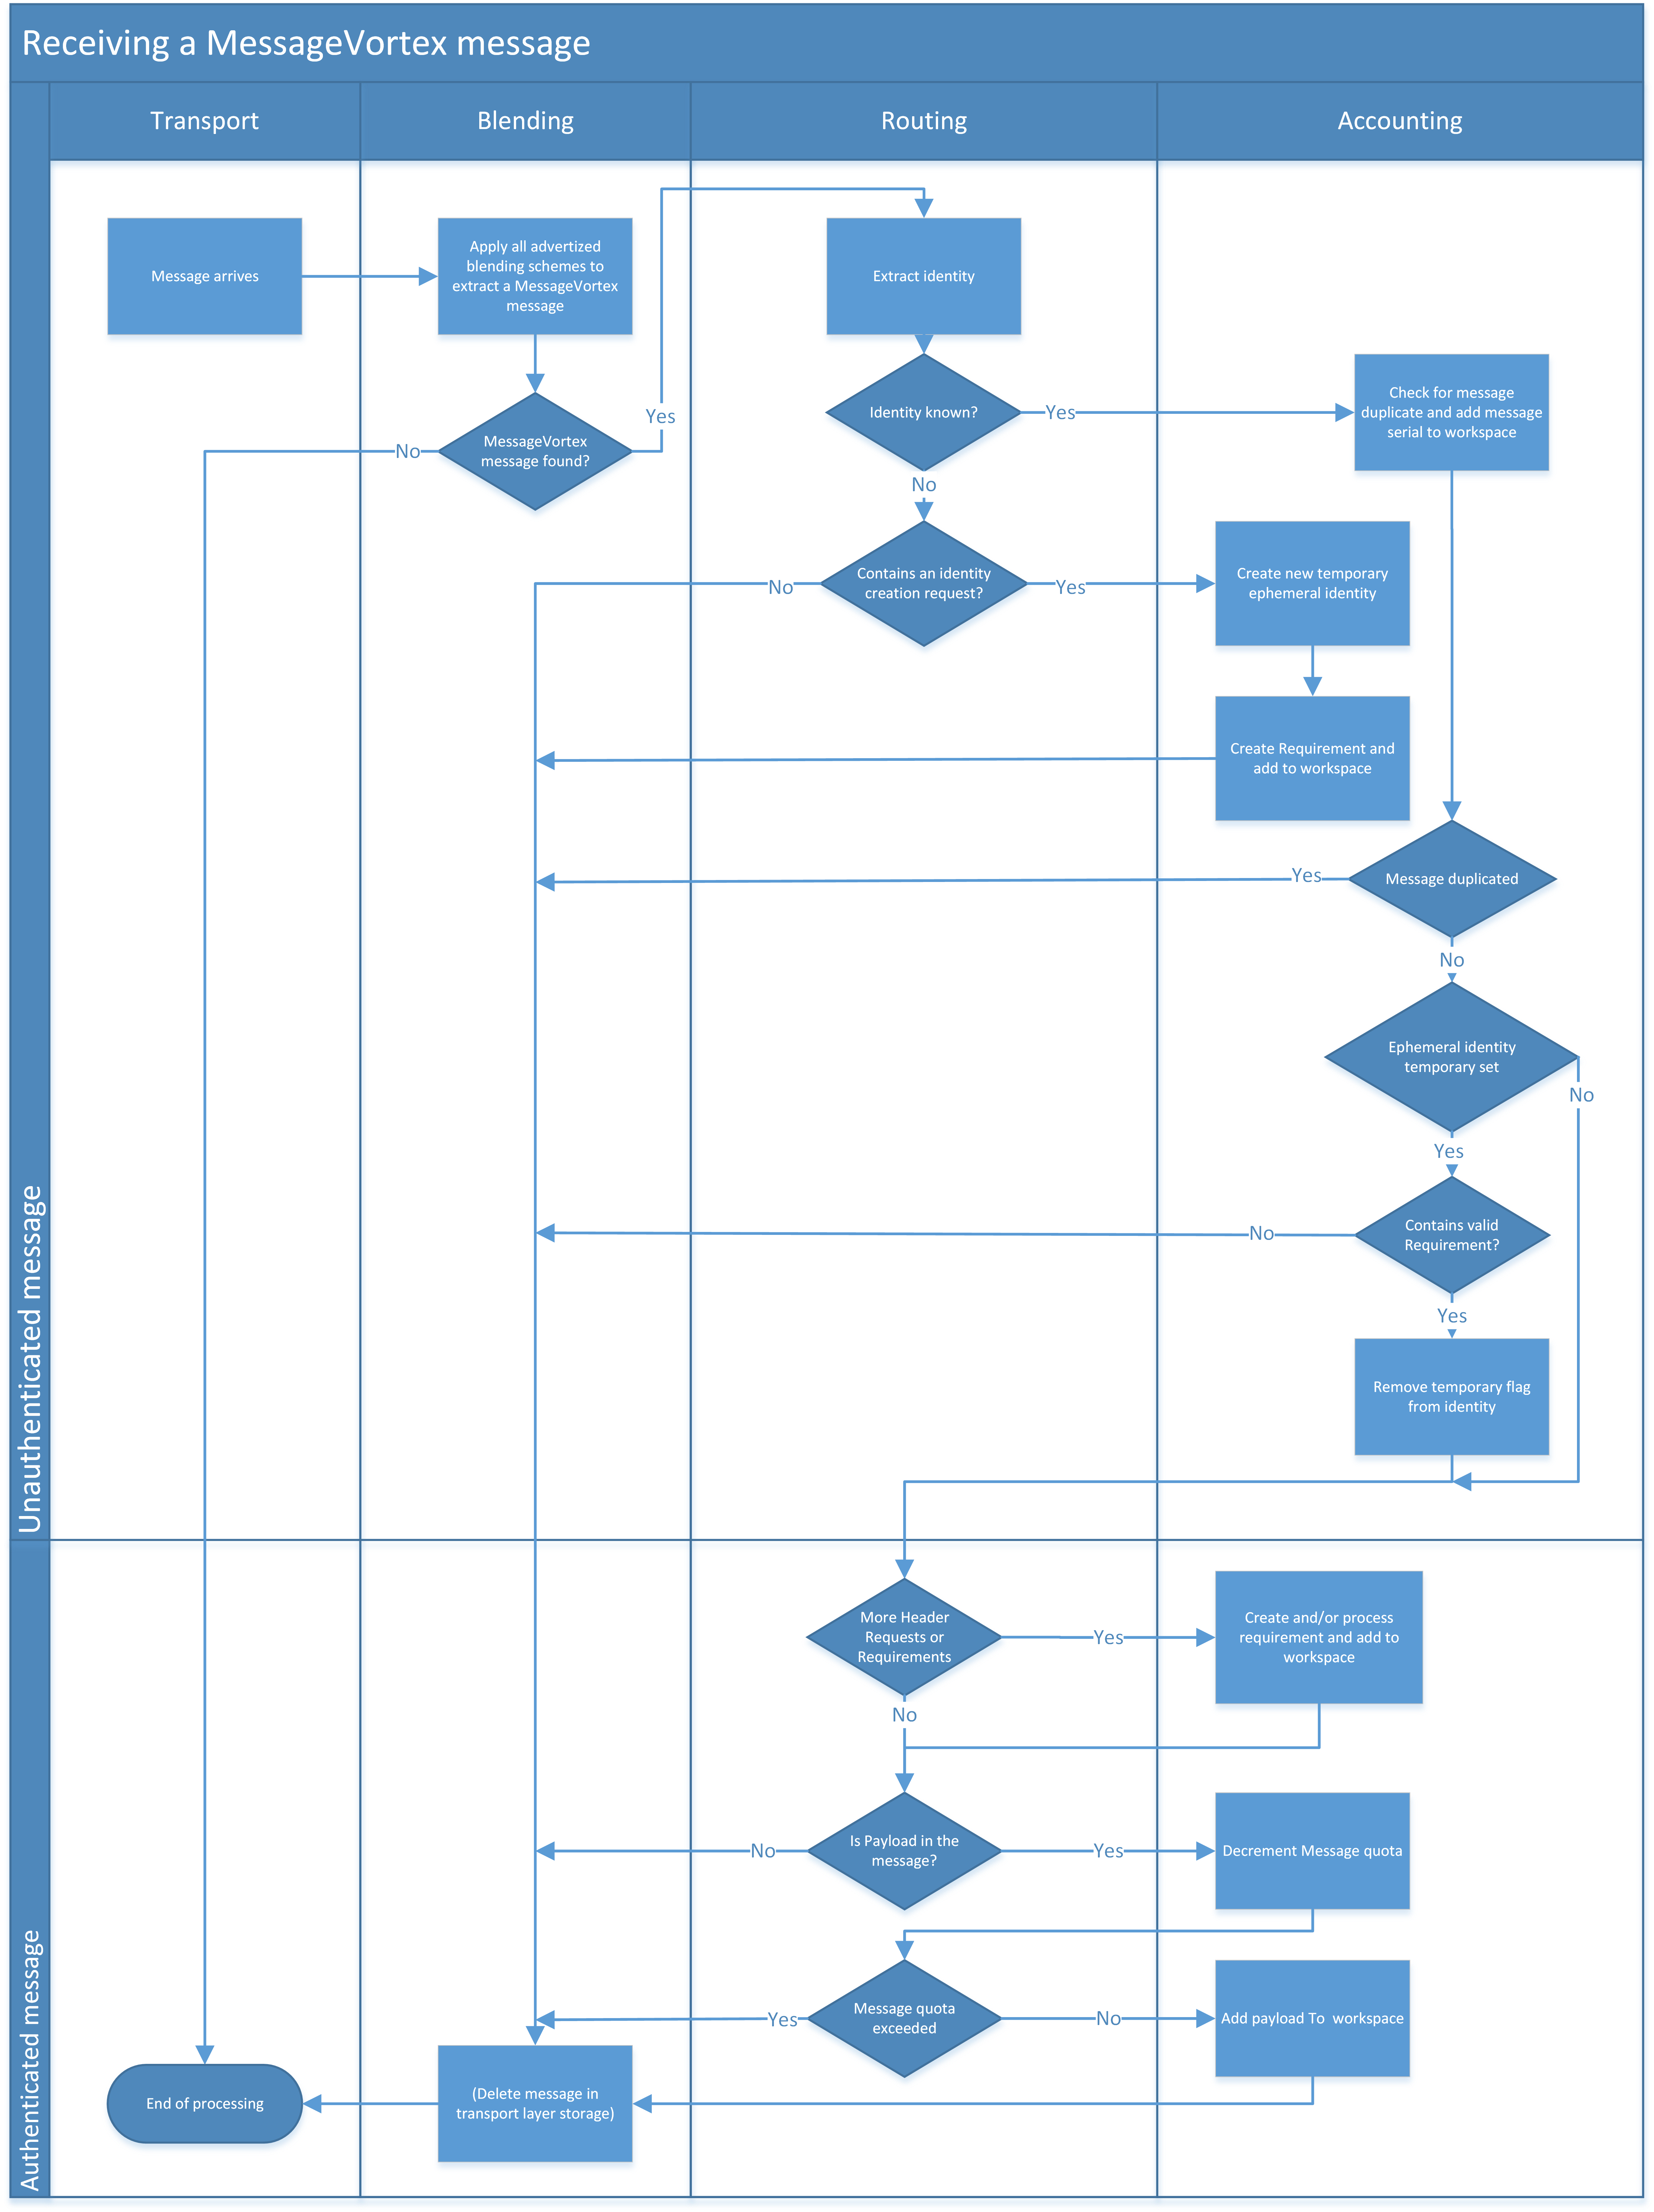
\includegraphics[width=\textwidth]{inc/flowchart_message_receiving}
	\caption{flow diagram showing processing of incomming messages}
	\label{fig:msgRecvProcessing}
\end{figure*}

\fxwarning{add content here}

\subsection{Transmission Block Processing}
\fxwarning{add content here}

\section{Sub Research Questions Roundup}
\subsection{SQ1: Sending messages maintaining unlikability against an adversary}
\fxwarning{add content here}
\subsection{SQ2: Attacking unlinkability and circumvention}
\fxwarning{add content here}
\subsection{SQ3: Attack Mitigation by design}
\fxwarning{add content here}

